\documentclass[12pt,oneside]{book}

%%%%%%%%%%%%%%%%%%%%%%%%%%%%%%%%%%%%%%%%%%%%%%%%%%%%%%%%%%%%%%%%%%%%%%%%%%%%%%%%%%%%%%%%%%%%%%%%%%%
%                                                                                                 %
% The mathematical style of these documents follows                                               %
%                                                                                                 %
% A. Thompson and B.N. Taylor. The NIST Guide for the Use of the International System of Units.   %
%    NIST Special Publication 881, 2008.                                                          %
%                                                                                                 %
% http://www.nist.gov/pml/pubs/sp811/index.cfm                                                    %
%                                                                                                 %
%%%%%%%%%%%%%%%%%%%%%%%%%%%%%%%%%%%%%%%%%%%%%%%%%%%%%%%%%%%%%%%%%%%%%%%%%%%%%%%%%%%%%%%%%%%%%%%%%%%

% $Date: 2013-11-26 10:43:59 -0500 (Tue, 26 Nov 2013) $
% $Revision: 17538 $
% $Author: gforney $

%%%%%%%%%%%%%%%%%%%%%%%%%%%%%%%%%%%%%%%%%%%%%%%%%%%%%%%%%%%%%%%%%%%%%%%%%%%%%%%%%%%%%%%%%%%%%%%%%%%
%                                                                                                 %
% The mathematical style of these documents follows                                               %
%                                                                                                 %
% A. Thompson and B.N. Taylor. The NIST Guide for the Use of the International System of Units.   %
%    NIST Special Publication 881, 2008.                                                          %
%                                                                                                 %
% http://www.nist.gov/pml/pubs/sp811/index.cfm                                                    %
%                                                                                                 %
%%%%%%%%%%%%%%%%%%%%%%%%%%%%%%%%%%%%%%%%%%%%%%%%%%%%%%%%%%%%%%%%%%%%%%%%%%%%%%%%%%%%%%%%%%%%%%%%%%%

% Packages which force the use of better TeX coding
% Mostly from http://tex.stackexchange.com/q/19264
%%\RequirePackage[l2tabu, orthodox]{nag}
%%\usepackage{fixltx2e}
%\usepackage{isomath} % Disabled for the moment because it changes the syntax for bold and roman Greek math symbols
%%\usepackage[all,warning]{onlyamsmath}
%\usepackage{strict} % Commented out for now because it is uncommon. A copy of style.sty is in Manuals/LaTeX_Style_Files/.

\usepackage{times,mathptmx}
\usepackage[pdftex]{graphicx}
\usepackage{tabularx,ragged2e,booktabs,caption}
\usepackage{multirow}
\usepackage{pdfsync}
\usepackage{tikz}
\usepackage{pgfplots}
%\pgfplotsset{compat=1.7}
\usepackage{tocloft}
\usepackage{color}
\usepackage{amsmath}
\definecolor{linknavy}{rgb}{0,0,0.50196}
\definecolor{linkred}{rgb}{1,0,0}
\definecolor{linkblue}{rgb}{0,0,1}
\usepackage{float}
\usepackage{caption}
\usepackage{graphpap}
\usepackage{rotating}
\usepackage{graphicx}
\usepackage{geometry}
\usepackage{relsize}
\usepackage{longtable}
\usepackage{lscape}
\usepackage{amssymb}
\usepackage{makeidx} % Create index at end of document
\usepackage[nottoc,notlof,notlot]{tocbibind} % Put the bibliography and index in the ToC
\usepackage{lastpage} % Automatic last page number reference.
\usepackage[T1]{fontenc}
\usepackage{enumerate}
\usepackage{upquote}
\usepackage{moreverb}
\usepackage{xfrac}
\usepackage{cite}

\newcommand{\nopart}{\expandafter\def\csname Parent-1\endcsname{}} % To fix table of contents in pdf.
\newcommand{\ct}{\tt\small} % eventually will be deprecated due to http://www.tex.ac.uk/cgi-bin/texfaq2html?label=2letterfontcmd
\newcommand{\textct}[1]{\texttt{\small #1}}

\usepackage{tocstyle} % Fix table of contents sections from overlapping section titles
\usetocstyle{standard}
\usepackage{siunitx}
\sisetup{
    detect-all = true,
    input-decimal-markers = {.},
    input-ignore = {,},
    inter-unit-product = \ensuremath{{}\cdot{}},
    multi-part-units = repeat,
    number-unit-product = \text{~},
    per-mode = fraction,
    separate-uncertainty = true,
}

\usepackage{listings}
\usepackage{textcomp}
\definecolor{lbcolor}{rgb}{0.96,0.96,0.96}
\lstset{
    %backgroundcolor=\color{lbcolor},
    tabsize=4,
    rulecolor=,
    language=Fortran,
        basicstyle=\footnotesize\ttfamily,
        upquote=true,
        aboveskip={\baselineskip},
        belowskip={\baselineskip},
        columns=fixed,
        extendedchars=true,
        breaklines=true,
        breakatwhitespace=true,
        frame=none,
        showtabs=false,
        showspaces=false,
        showstringspaces=false,
        identifierstyle=\ttfamily,
        keywordstyle=\color[rgb]{0,0,0},
        commentstyle=\color[rgb]{0,0,0},
        stringstyle=\color[rgb]{0,0,0},
}

\usepackage[pdftex,
        colorlinks=true,
        urlcolor=linkblue,     % \href{...}{...} external (URL)
        citecolor=linkred,     % citation number colors
        linkcolor=linknavy,    % \ref{...} and \pageref{...}
        pdfproducer={pdflatex},
        pdfpagemode=UseNone,
        bookmarksopen=true,
        plainpages=false,
        verbose]{hyperref}

% The Following commented code makes the ``Draft'' watermark on each page.
%\usepackage{eso-pic}
%\usepackage{type1cm}
%\makeatletter
%   \AddToShipoutPicture{
%     \setlength{\@tempdimb}{.5\paperwidth}
%     \setlength{\@tempdimc}{.5\paperheight}
%     \setlength{\unitlength}{1pt}
%     \put(\strip@pt\@tempdimb,\strip@pt\@tempdimc){
%     \makebox(0,0){\rotatebox{45}{\textcolor[gray]{0.75}{\fontsize{8cm}\selectfont{RC6}}}}}
% }
%\makeatother

\setlength{\textwidth}{6.5in}
\setlength{\textheight}{9.0in}
\setlength{\topmargin}{0.in}
\setlength{\headheight}{0.pt}
\setlength{\headsep}{0.in}
\setlength{\parindent}{0.25in}
\setlength{\oddsidemargin}{0.0in}
\setlength{\evensidemargin}{0.0in}
\setlength{\leftmargini}{\parindent} % Controls the indenting of the "bullets" in a list
\setlength{\cftsecnumwidth}{0.45in}
\setlength{\cftsubsecnumwidth}{0.5in}
\setlength{\cftfignumwidth}{0.45in}
\setlength{\cfttabnumwidth}{0.45in}

\newcommand{\titlesigs}
{
\small
\flushright{U.S. Department of Commerce \\
{\em Penny Pritzker, Secretary} \\
\hspace{1in} \\
National Institute of Standards and Technology \\
{\em Willie May, Under Secretary of Commerce for Standards and Technology and Acting Director} }
}

% commands to use for "official" cover and title pages
% see smokeview verification guide to see how they are used

\newcommand{\headerA}[1]{
\flushright{
\fontsize{20}{24}\selectfont
\bf{NIST Special Publication #1}}
}

\newcommand{\headerB}[1]{
\flushright{
\fontsize{28}{33.6}\selectfont
\bf{#1}
}
}

\newcommand{\headerC}[1]{
\vspace{.5in}
\flushright{\fontsize{14}{16.8}\selectfont
#1}
}

\frenchspacing

\newcommand{\dod}[2]{\frac{\partial #1}{\partial #2}}
\newcommand{\DoD}[2]{\frac{\mathrm{D} #1}{\mathrm{D} #2}}
\newcommand{\dsods}[2]{\frac{\partial^2 #1}{\partial #2^2}}
\renewcommand{\d}{\,\mathrm{d}}
\newcommand{\dx}{\delta x}
\newcommand{\dy}{\delta y}
\newcommand{\dz}{\delta z}
\newcommand{\degF}{$^\circ$F}
\newcommand{\degC}{$^\circ$C}
\newcommand{\x}{x}
\newcommand{\y}{y}
\newcommand{\z}{z}
\newcommand{\dt}{\delta t}
\newcommand{\dn}{\delta n}
\newcommand{\cH}{H}
\newcommand{\hu}{u}
\newcommand{\hv}{v}
\newcommand{\hw}{w}
\newcommand{\la}{\lambda}
\newcommand{\bO}{{\Omega}}
\newcommand{\bo}{{\mathbf{\omega}}}
\newcommand{\btau}{\mathbf{\tau}}
\newcommand{\bdelta}{{\mathbf{\delta}}}
\newcommand{\sumyw}{\sum (Y_\alpha/W_\alpha)}
\newcommand{\oW}{\overline{W}}
\newcommand{\om}{\ensuremath{\omega}}
\newcommand{\omx}{\omega_x}
\newcommand{\omy}{\omega_y}
\newcommand{\omz}{\omega_z}
\newcommand{\erf}{\hbox{erf}}
\newcommand{\erfc}{\hbox{erfc}}
\newcommand{\bF}{{\mathbf{F}}}
\newcommand{\bG}{{\mathbf{G}}}
\newcommand{\bof}{{\mathbf{f}}}
\newcommand{\bq}{{\mathbf{q}}}
\newcommand{\br}{{\mathbf{r}}}
\newcommand{\bu}{{\mathbf{u}}}
\newcommand{\bx}{{\mathbf{x}}}
\newcommand{\bk}{{\mathbf{k}}}
\newcommand{\bv}{{\mathbf{v}}}
\newcommand{\bg}{{\mathbf{g}}}
\newcommand{\bn}{{\mathbf{n}}}
\newcommand{\bS}{{\mathbf{S}}}
\newcommand{\bW}{\overline{W}}
\newcommand{\dS}{d{\mathbf{S}}}
\newcommand{\bs}{{\mathbf{s}}}
\newcommand{\bI}{{\mathbf{I}}}
\newcommand{\hp}{H}
\newcommand{\trho}{\tilde{\rho}}
\newcommand{\dph}{{\delta\phi}}
\newcommand{\dth}{{\delta\theta}}
\newcommand{\tp}{\tilde{p}}
\newcommand{\bp}{\overline{p}}
\newcommand{\dQ}{\dot{Q}}
\newcommand{\dq}{\dot{q}}
\newcommand{\dbq}{\dot{\mathbf{q}}}
\newcommand{\dm}{\dot{m}}
\newcommand{\ha}{\frac{1}{2}}
\newcommand{\ft}{\frac{4}{3}}
\newcommand{\ot}{\frac{1}{3}}
\newcommand{\fofi}{\frac{4}{5}}
\newcommand{\of}{\frac{1}{4}}
\newcommand{\twth}{\frac{2}{3}}
\newcommand{\R}{R}
\newcommand{\be}{\begin{equation}}
\newcommand{\ee}{\end{equation}}
\newcommand{\RE}{\hbox{Re}}
\newcommand{\LE}{\hbox{Le}}
\newcommand{\PR}{\hbox{Pr}}
\newcommand{\PE}{\hbox{Pe}}
\newcommand{\NU}{\hbox{Nu}}
\newcommand{\SC}{\hbox{Sc}}
\newcommand{\SH}{\hbox{Sh}}
\newcommand{\WE}{\hbox{We}}
\newcommand{\COTWO}{\text{\tiny \hbox{CO}$_2$}}
\newcommand{\HTWOO}{\text{\tiny \hbox{H}$_2$\hbox{O}}}
\newcommand{\OTWO}{\text{\tiny \hbox{O}$_2$}}
\newcommand{\NTWO}{\text{\tiny \hbox{N}$_2$}}
\newcommand{\CO}{\text{\tiny \hbox{CO}}}
\newcommand{\F}{\text{\tiny \hbox{F}}}
\newcommand{\C}{\text{\tiny \hbox{C}}}
\newcommand{\Hy}{\text{\tiny \hbox{H}}}
\newcommand{\So}{\text{\tiny \hbox{S}}}
\newcommand{\M}{\text{\tiny \hbox{M}}}
\newcommand{\xx}{\text{\tiny \hbox{x}}}
\newcommand{\yy}{\text{\tiny \hbox{y}}}
\newcommand{\zz}{\text{\tiny \hbox{z}}}
\newcommand{\smvlines}{115~000}

\newcommand{\calH}{\mathcal{H}}
\newcommand{\calR}{\mathcal{R}}

\newcommand{\dif}{\mathrm{d}}
\newcommand{\Div}{\nabla\cdot}
\newcommand{\D}{\mbox{D}}
\newcommand{\mhalf}{\mbox{$\frac{1}{2}$}}
\newcommand{\thalf}{\mbox{\tiny $\frac{1}{2}$}}
\newcommand{\tripleprime}{{\prime\prime\prime}}
\newcommand{\ppp}{{\prime\prime\prime}}
\newcommand{\pp}{{\prime\prime}}

\newcommand{\superscript}[1]{\ensuremath{^{\textrm{\tiny #1}}}}
\newcommand{\subscript}[1]{\ensuremath{_{\textrm{\tiny #1}}}}

\newcommand{\rb}[1]{\raisebox{1.5ex}[0pt]{#1}}

\newcommand{\Ra}{$\Rightarrow$}
\newcommand{\hhref}[1]{\href{#1}{{\tt #1}}}
\newcommand{\fdsinput}[1]{{\scriptsize\verbatiminput{../../Verification/Visualization/#1}}}

\definecolor{AQUAMARINE}{rgb}{0.49804,1.00000,0.83137}
\definecolor{ANTIQUE WHITE}{rgb}{0.98039,0.92157,0.84314}
\definecolor{BEIGE}{rgb}{0.96078,0.96078,0.86275}
\definecolor{BLACK}{rgb}{0.00000,0.00000,0.00000}
\definecolor{BLUE}{rgb}{0.00000,0.00000,1.00000}
\definecolor{BLUE VIOLET}{rgb}{0.54118,0.16863,0.88627}
\definecolor{BRICK}{rgb}{0.61176,0.40000,0.12157}
\definecolor{BROWN}{rgb}{0.64706,0.16471,0.16471}
\definecolor{BURNT SIENNA}{rgb}{0.54118,0.21176,0.05882}
\definecolor{BURNT UMBER}{rgb}{0.54118,0.20000,0.14118}
\definecolor{CADET BLUE}{rgb}{0.37255,0.61961,0.62745}
\definecolor{CHOCOLATE}{rgb}{0.82353,0.41176,0.11765}
\definecolor{COBALT}{rgb}{0.23922,0.34902,0.67059}
\definecolor{CORAL}{rgb}{1.00000,0.49804,0.31373}
\definecolor{CYAN}{rgb}{0.00000,1.00000,1.00000}
\definecolor{DIMGRAY }{rgb}{0.41176,0.41176,0.41176}
\definecolor{EMERALD GREEN}{rgb}{0.00000,0.78824,0.34118}
\definecolor{FIREBRICK}{rgb}{0.69804,0.13333,0.13333}
\definecolor{FLESH}{rgb}{1.00000,0.49020,0.25098}
\definecolor{FOREST GREEN}{rgb}{0.13333,0.54510,0.13333}
\definecolor{GOLD }{rgb}{1.00000,0.84314,0.00000}
\definecolor{GOLDENROD}{rgb}{0.85490,0.64706,0.12549}
\definecolor{GRAY}{rgb}{0.50196,0.50196,0.50196}
\definecolor{GREEN}{rgb}{0.00000,1.00000,0.00000}
\definecolor{GREEN YELLOW}{rgb}{0.67843,1.00000,0.18431}
\definecolor{HONEYDEW}{rgb}{0.94118,1.00000,0.94118}
\definecolor{HOT PINK}{rgb}{1.00000,0.41176,0.70588}
\definecolor{INDIAN RED}{rgb}{0.80392,0.36078,0.36078}
\definecolor{INDIGO}{rgb}{0.29412,0.00000,0.50980}
\definecolor{IVORY}{rgb}{1.00000,1.00000,0.94118}
\definecolor{IVORY BLACK}{rgb}{0.16078,0.14118,0.12941}
\definecolor{KELLY GREEN}{rgb}{0.00000,0.50196,0.00000}
\definecolor{KHAKI}{rgb}{0.94118,0.90196,0.54902}
\definecolor{LAVENDER}{rgb}{0.90196,0.90196,0.98039}
\definecolor{LIME GREEN}{rgb}{0.19608,0.80392,0.19608}
\definecolor{MAGENTA}{rgb}{1.00000,0.00000,1.00000}
\definecolor{MAROON}{rgb}{0.50196,0.00000,0.00000}
\definecolor{MELON}{rgb}{0.89020,0.65882,0.41176}
\definecolor{MIDNIGHT BLUE}{rgb}{0.09804,0.09804,0.43922}
\definecolor{MINT}{rgb}{0.74118,0.98824,0.78824}
\definecolor{NAVY}{rgb}{0.00000,0.00000,0.50196}
\definecolor{OLIVE}{rgb}{0.50196,0.50196,0.00000}
\definecolor{OLIVE DRAB}{rgb}{0.41961,0.55686,0.13725}
\definecolor{ORANGE}{rgb}{1.00000,0.50196,0.00000}
\definecolor{ORANGE RED}{rgb}{1.00000,0.27059,0.00000}
\definecolor{ORCHID}{rgb}{0.85490,0.43922,0.83922}
\definecolor{PINK}{rgb}{1.00000,0.75294,0.79608}
\definecolor{POWDER BLUE}{rgb}{0.69020,0.87843,0.90196}
\definecolor{PURPLE}{rgb}{0.50196,0.00000,0.50196}
\definecolor{RASPBERRY}{rgb}{0.52941,0.14902,0.34118}
\definecolor{RED}{rgb}{1.00000,0.00000,0.00000}
\definecolor{ROYAL BLUE}{rgb}{0.25490,0.41176,0.88235}
\definecolor{SALMON}{rgb}{0.98039,0.50196,0.44706}
\definecolor{SANDY BROWN}{rgb}{0.95686,0.64314,0.37647}
\definecolor{SEA GREEN}{rgb}{0.32941,1.00000,0.62353}
\definecolor{SEPIA}{rgb}{0.36863,0.14902,0.07059}
\definecolor{SIENNA}{rgb}{0.62745,0.32157,0.17647}
\definecolor{SILVER}{rgb}{0.75294,0.75294,0.75294}
\definecolor{SKY BLUE}{rgb}{0.52941,0.80784,0.92157}
\definecolor{SLATEBLUE}{rgb}{0.41569,0.35294,0.80392}
\definecolor{SLATE GRAY}{rgb}{0.43922,0.50196,0.56471}
\definecolor{SPRING GREEN}{rgb}{0.00000,1.00000,0.49804}
\definecolor{STEEL BLUE}{rgb}{0.27451,0.50980,0.70588}
\definecolor{TAN}{rgb}{0.82353,0.70588,0.54902}
\definecolor{TEAL}{rgb}{0.00000,0.50196,0.50196}
\definecolor{THISTLE}{rgb}{0.84706,0.74902,0.84706}
\definecolor{TOMATO }{rgb}{1.00000,0.38824,0.27843}
\definecolor{TURQUOISE}{rgb}{0.25098,0.87843,0.81569}
\definecolor{VIOLET}{rgb}{0.93333,0.50980,0.93333}
\definecolor{VIOLET RED}{rgb}{0.81569,0.12549,0.56471}
\definecolor{WHITE}{rgb}{1.00000,1.00000,1.00000}
\definecolor{YELLOW}{rgb}{1.00000,1.00000,0.00000}

\pgfplotsset{
	colormap={blackwhite}{[5pt]
		rgb255(0pt)=(0,0,255); 
		rgb255(100pt)=(0,255,255); 
		rgb255(200pt)=(0,255,0); 
		rgb255(300pt)=(255,255,0); 
		rgb255(400pt)=(255,0,0)
	},
} % defines smokeview colorbar


\floatstyle{boxed}
\newfloat{notebox}{H}{lon}
\newfloat{warning}{H}{low}

% Set default longtable alignment
\setlength\LTleft{0pt}
\setlength\LTright{0pt}


% Rename chapter headings
\renewcommand{\chaptername}{Section}
\renewcommand{\bibname}{References}

% Math shortcuts
\renewcommand{\sb}[1]{_\mathrm{#1}}
\renewcommand{\C}{\mbox{C}}
\renewcommand{\H}{\mbox{H}}
\renewcommand{\O}{\mbox{O}}
\newcommand{\N}{\mbox{N}}

% Center all figures
\makeatletter
\g@addto@macro\@floatboxreset\centering
\makeatother

% Extra packages
\usepackage{xfrac}

\begin{document}

\bibliographystyle{unsrt}
\pagestyle{empty}

\begin{minipage}[t][9in][s]{6.25in}

\begin{flushright}
\fontsize{20}{24}\selectfont
\bf{NIST Technical Note XXXX}
\end{flushright}

\headerB{
Examination of Compressed Air Foam (CAF) for Interior Firefighting \\
Spring 2012 \\
}

\normalsize

\headerC{
{
\flushright{
Craig G. Weinschenk \\
Keith M. Stakes \\
Daniel Madrzykowski \\

\vspace*{2\baselineskip}

\begingroup
This publication is available free of charge from:
\hypersetup{urlcolor=black}
\href{http://dx.doi.org/10.6028/NIST.TN.XXXX}{http://dx.doi.org/10.6028/NIST.TN.XXXX}
\endgroup
}

\vfill

\flushright{


\includegraphics[width=2.in]{../../../Bibliography/nistident_flright_vec} \\[.3in]
}
}
}

\end{minipage}

\newpage
\hspace{5in}
\newpage

\frontmatter

\pagenumbering{roman}

\begin{minipage}[t][9in][s]{6.25in}

\begin{flushright}
\fontsize{20}{24}\selectfont
\bf{NIST Technical Note XXXX}
\end{flushright}

\headerB{
Examination of Compressed Air Foam (CAF) for Interior Firefighting \\
Spring 2012 \\
}

\headerC{
\flushright{
Craig G. Weinschenk \\
Keith M. Stakes \\
Daniel Madrzykowski \\
{\em Fire Research Division \\
Engineering Laboratory} \\

\vspace*{2\baselineskip}

\begingroup
This publication is available free of charge from:
\hypersetup{urlcolor=black}
\href{http://dx.doi.org/10.6028/NIST.TN.XXXX}{http://dx.doi.org/10.6028/NIST.TN.XXXX} \\
\endgroup

\vspace*{2\baselineskip}
August 2015}}

\vfill

\flushright{
\includegraphics[width=1in]{../../../Bibliography/doc} }

\titlesigs

\end{minipage}

\newpage

\begin{minipage}[t][9in][s]{6.25in}

\flushright{Certain commercial entities, equipment, or materials may be identified in this \\
document in order to describe an experimental procedure or concept adequately. \\
Such identification is not intended to imply recommendation or endorsement by the \\
National Institute of Standards and Technology, nor is it intended to imply that the \\
entities, materials, or equipment are necessarily the best available for the purpose. \\
}

\vspace{3in}

\large
\flushright{\bf National Institute of Standards and Technology Technical Note XXXX \\
Natl.~Inst.~Stand.~Technol.~Tech.~Note~XX, \pageref{LastPage} pages (August 2015) \\
% http://dx.doi.org/10.6028/NIST.TN.XXXX \\
CODEN: NTNOEF }

\vspace{0.2in}

\begingroup
{\bf This publication is available free of charge from:}
\hypersetup{urlcolor=black}
\href{http://dx.doi.org/10.6028/NIST.TN.1838}{\bf http://dx.doi.org/10.6028/NIST.TN.1838} \\
\endgroup

\vfill

\hspace{1in}

\end{minipage}

\newpage

\frontmatter

\pagestyle{plain}
\pagenumbering{roman}

\cleardoublepage
\phantomsection
\addcontentsline{toc}{chapter}{Contents}
\tableofcontents

\cleardoublepage
\phantomsection
\addcontentsline{toc}{chapter}{List of Figures}
\listoffigures

\cleardoublepage
\phantomsection
\addcontentsline{toc}{chapter}{List of Tables}
\listoftables

\chapter{List of Acronyms}

\begin{tabbing}
\hspace{1.5in} \= \\
ESTC \> Delaware County Emergency Services Training Center \\
MCFRS \> Montgomery County (MD) Fire and Rescue Service \\
NIST \> National Institute of Standards and Technology \\
TFT \> Task Force Tips \\
\end{tabbing}

\mainmatter

\chapter*{\centering Abstract}
Traditionally, fire fighting suppression operations have been conducted from the interior of the structure as a means to reduce water damage, manage the ``thermal balance'', and limit fire damage to structures. In current fire fighter training manuals, it is stated that these operations must be coordinated with the ventilation operations. However guidance on that coordination has been limited. Previous research and examinations of line of duty deaths have shown that ventilation events occurring with fire fighters in the structure prior to suppression have led to tragic results. One means of reducing the possibilities of this occurrence would be to begin to extinguish the fire prior to entering the structure. In effect, an offensive, exterior fire attack, in which water is directed into the structure from the exterior to cool the fire gases and reduce the heat release rate of the fire, prior to the fire fighters entering the building. The major concern with this type of operation is the potential harm that might occur to people trapped in the structure or the amount of water damage to the structure. Additionally, the type of suppression agent can affect the fire behavior within the structure. The suppression agent is the main focus of this study to determine whether or not compressed air foam systems provide any significant benefit to the traditional water application. Therefore, measurements are needed to document the changes of the thermal environment within the structure due to interior and exterior fire suppression tactics over all types of suppression agents. This report will focus on water distribution and fire suppression experiments conducted to develop a baseline for the interior fire suppression using both water and compressed air foam application.
\pagenumbering{gobble}

\chapter{Introduction}
\label{chap:Introduction}
 \pagenumbering{arabic}
\setcounter{page}{1}

The Engineering Laboratory at the National Institute of Standards and Technology (NIST) has a research program aimed at improving the safety and effectiveness of firefighters through improved knowledge of fire behavior and firefighting tactics. One of the objectives of this program is to examine non-traditional means of fire suppression. This series of experiments conducted by NIST for the California Polytechnic State University (Cal Poly), San Luis Obispo in collaboration with the Montgomery County (MD) Fire and Rescue Service complements the NIST research program on firefighting tactics. These experiments are part of a larger research project led by Cal Poly with the purpose of investigating the capabilities and limitations of compressed air foam systems (CAFS) for structural firefighting with the objective of enhancing the scientific knowledge base regarding the effectiveness and safety implications associated with the use of CAFS for structural firefighting.

NIST conducted several series of experiments to provide scientific measurements and comparisons between CAFS and water-only hose streams for different compartment fire scenarios.

Three types of experiments were conducted:
\begin{enumerate}
\item spray density measures under non-fire conditions
\item gas layer cooling
\item fire suppression in experimental structures
\end{enumerate}

The key measures were to understand the cooling and suppression capabilities of CAFS compared to water. The experimental designs were developed based on a project planning workshop which included the discussion of incidents where firefighters had concerns or experienced minor burns while using CAFS during interior attack operations in residential occupancies~\cite{Grant:2011}.

Since Montgomery County (MD) Fire and Rescue Service (MCFRS) provided the CAFS equipped engines and the staffing needed to provide both the water and CAF for the experiments. Baseline operating conditions were agreed upon at the workshop for these experiments (Table~\ref{tab:op_condition}). These experiments were conducted at the Delaware County Emergency Services Training Center (ESTC) in Sharon Hill, PA.

\begin{table}[!ht]
\centering
\captionof{table}{Operating conditions for experiments}\label{tab:op_condition}
\begin{tabular}{ll}
\toprule[1.5pt]
Equipment    &   Operating Condition \\
\midrule
Nozzle       & Metro 1, fixed gallonage fog, straight, or 7/8~inch solid stream \\
Hoseline     & 100~ft of 1-3/4~inch hoseline \\
Foam         & 0.3\% foam concentration \\
Pressure     & Water and Air pressure of 100 - 120~psi \\
\bottomrule[1.25pt]
\end{tabular}\par
\end{table}


\chapter{Experimental Setup}

\section{Description of Experiments}
\label{sec:desc_experiments}
The experimental setup for this test series is described by the three types of experiments conducted: spray density measures, gas layer cooling, and fire suppression. The nozzles chosen for these experiments were decided upon during the CAFS workshop~\cite{Grant:2011}: Task Force Tips (TFT) Metro 1, fixed gallonage nozzles with a flow rate of 120 gpm. These are automatic nozzles which have a 7/8~inch slug-tip and can be varied from a straight stream to a wide fog for application. The set-up also included 100~ft of 1-3/4~inch hose. Nozzles were mounted to a ``blitz-fire'' monitor device and placed inside the structures. The nozzles were controlled and operated via a gate valve from the exterior.

\subsection{Spray Density}
\label{sec:desc_Spray_Density}

Thirty-two tests were conducted to determine spray density measures based on various nozzle patterns and locations. The gas cooling and fire suppression tests simulated an interior fire attack through the deployment of hose lines inside the structures with fixed nozzles. Therefore, the purpose of these tests was to determine the appropriate nozzle locations for the gas cooling and fire suppression tests to follow by gaining an understanding of the water distribution throughout the structures.

Twenty-one of the tests were conducted in the concrete burn building where the gas cooling tests would take place, and twelve of the tests were conducted in the experimental structures to be used for the fire suppression tests. The test variables were the nozzle height, nozzle location within the test structure, and the nozzle pattern (cf. Fig.~\ref{fig:Spray_Density_Nozzle_Patterns}). A description and drawings of these facilities are included in Section~\ref{sec:Experimental Structures}. Detailed discussion of the tests and results are in Section~\ref{sec:Spray_Density}.

\begin{figure}[!ht]
	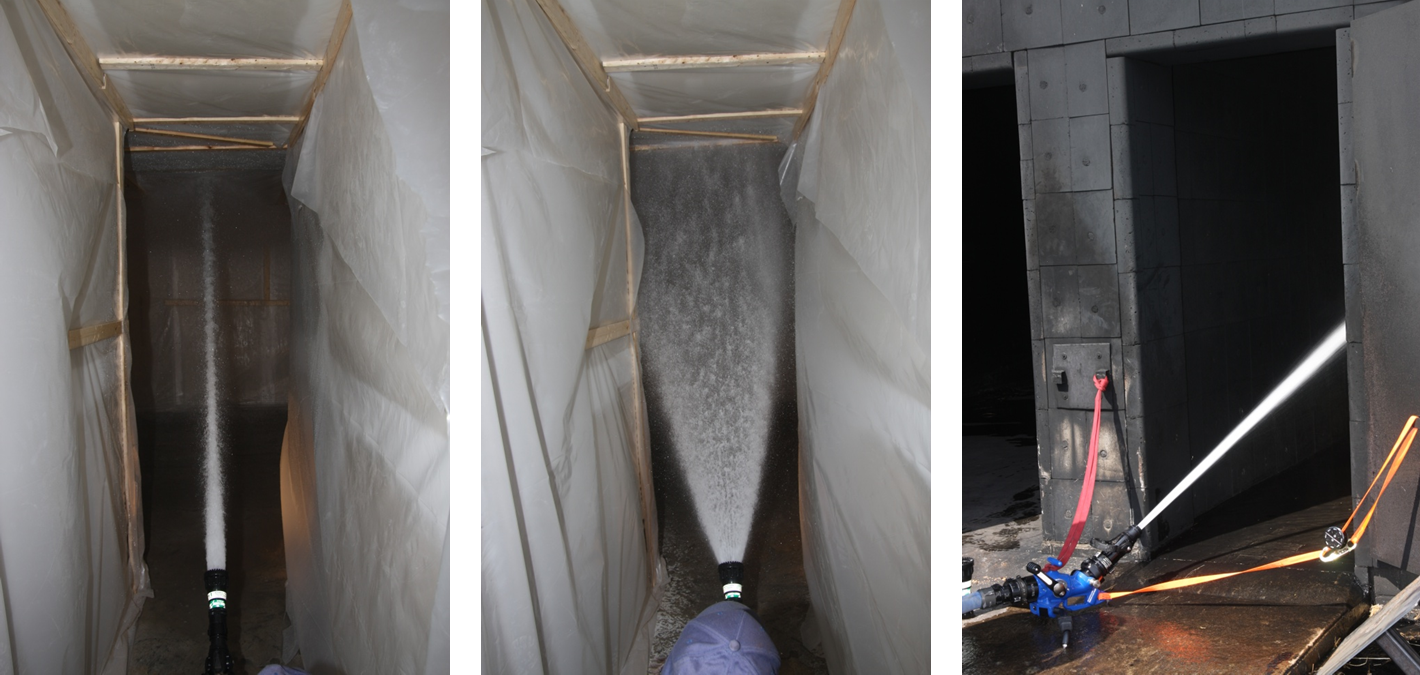
\includegraphics[width=6in]{../Figures/Pictures/Flows}
	\caption{Spray Density Nozzle Patterns}
	\label{fig:Spray_Density_Nozzle_Patterns}
\end{figure}

\subsection{Gas Cooling}
\label{sec:desc_Gas_Cooling}

Eighty-eight experiments were conducted to study the effectiveness of cooling the upper gas layer in a space adjacent to the area of fire involvement. These tests examined five different hose stream patterns, two nozzle types, and both compressed air foam and water as the suppression agent. The focus of this experimental series was to study the impact of the test variables on interior conditions throughout the structure when suppression tactics were applied to a room adjacent to the fire room. Detailed discussion of the tests and results are in Section~\ref{sec:Gas_Cooling}.

\subsection{Fire Suppression}
\label{sec:desc_Fire_Suppression}

The fire suppression series included 14 tests in two single-story experimental structures. Six tests were conducted in the East structure and six tests were conducted in the West structure, each including both water and CAF application as a suppression agent. The nozzle patterns were varied from straight stream to narrow fog. Two additional tests were conduction on suppression tactics for attic fires in residential dwellings, one in each structure. For these tests, a smooth bore nozzle was used.

\section{Experimental Facilities}
\label{sec:Experimental_Facility}

The series of tests described within this report were conducted at the Delaware County Emergency Services Training Center, located in Sharon Hill, PA. A burn building as well as two purpose built concrete structures are located on the grounds of the ESTC. The burn building was used for the gas cooling experiments and the purpose built concrete structures were used for the fire suppression experiments.

\subsection{Fire Training Structure}
\label{sec:Burn_Building}

The burn building is a live fire training structure with both a two story and three story section. The building is supported with reinforced concrete beams and columns. The floors and ceilings are also concrete with the interior walls constructed of cement block. The walls and ceiling of the burn rooms are protected with a 25~mm thick layer of calcium silicate insulation and is covered by a 50~mm thick concrete tile. The floor of the burn rooms is protected with fire brick. Tests were conducted in the two-story, two-room configuration which has overall dimensions of 6.5~m (21.3~ft) by 9.2~m (30.2~ft) (cf. Fig.~\ref{fig:Delaware_County,_PA_Burn_Building_Layout}).

\begin{figure}[!ht]
	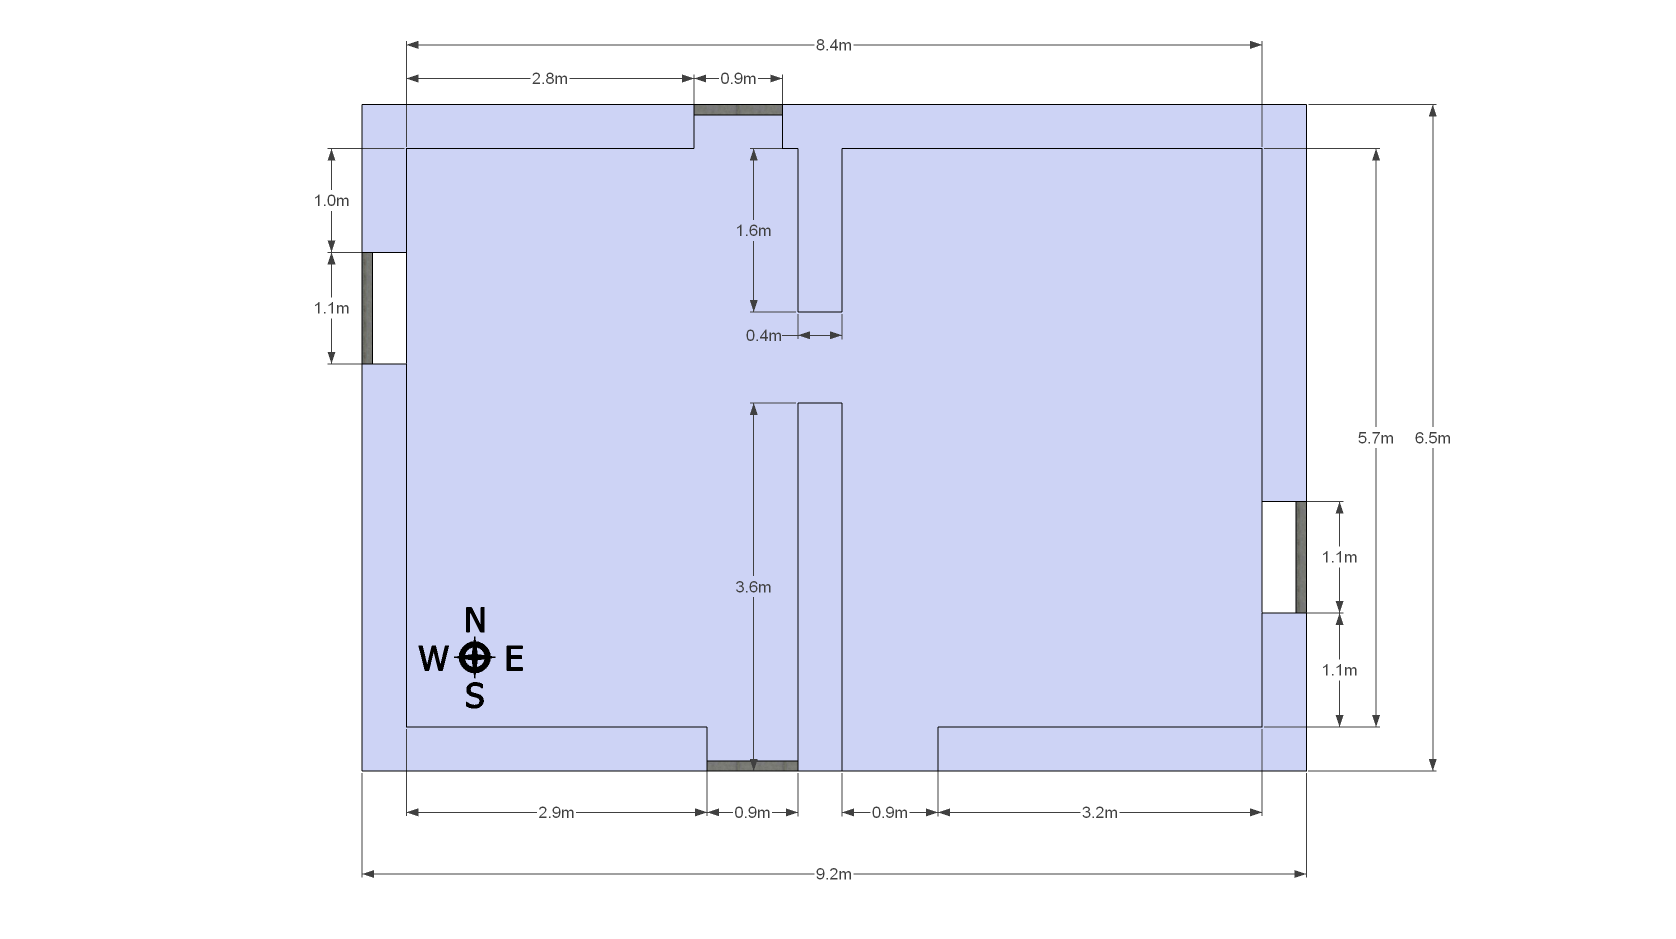
\includegraphics[width=6in]{../Figures/Pictures/DelCoBurnBuildingDimensions}
	\caption{Delaware County, PA Burn Building Layout}
	\label{fig:Delaware_County,_PA_Burn_Building_Layout}
\end{figure}

The burn room where the fuel load was located measured 3.8~m (12.5~ft) by 5.7~m (18.7~ft) with a ceiling height of 3.35~m (11.0~ft). The adjacent room where the water was applied for gas cooling measured 4.1~m (13.4~ft) by 5.7~m (18.7~ft), also with a ceiling height of 3.35~m (11.0~ft). The open door from the adjacent room to the exterior measured 2.0~m (6.5~ft) high and 0.9~m (2.9~ft) wide.

\subsection{Concrete Block Structures}
\label{sec:Experimental Structures}

Two identical concrete structures were built on a concrete slab as shown in Fig.~\ref{fig:Delaware_County,_PA_Fire_Test_Structures}. They were designed to simulate a single floor of a residential structure.  The outer wall of each structure was composed of interlocking concrete blocks 0.61~m (2~ft) wide, 0.61~m (2~ft) high and 1.22~m (4~ft) long.  The interior dimensions of each structure were 6.1~m (20~ft) wide, 11~m (36~ft) long and 2.4~m (8~ft) high. The joints and gaps between the blocks were filled with high temperature insulation.

\begin{figure}[!ht]
	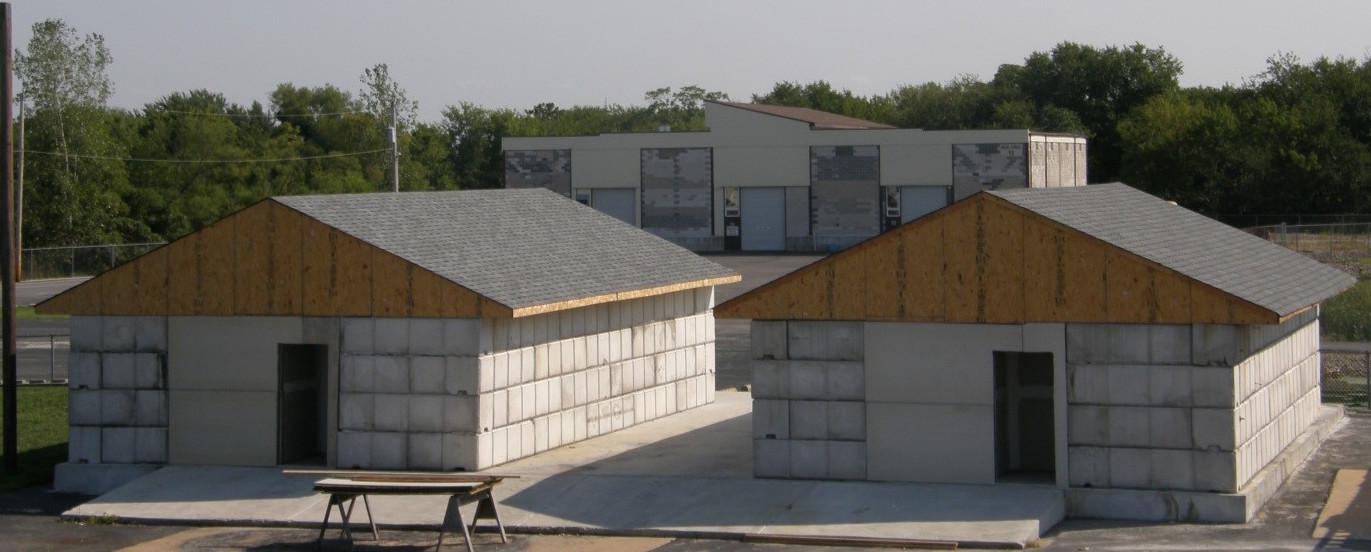
\includegraphics[width=6in]{../Figures/Pictures/DelCo_Structures}
	\caption{Delaware County, PA Fire Test Structures}
	\label{fig:Delaware_County,_PA_Fire_Test_Structures}
\end{figure}

Each structure had burn room, approximately 6.0~m (19.6~ft) by 4.4~m (14.3~ft) and 2.74~m (9.0~ft) in height and a hallway connecting the burn room to the front of the structure via a small entry foyer. The hallway was 0.95~m (3.1~ft) wide and 5.4~m (17.6~ft) long and the entry foyer was 1.2~m (4.1~ft) by 1.9~m (6.1~ft). The ceiling height in the hallway and entry foyer was 2.4~m (8~ft).  The open door on north side from the exterior to the entry foyer was 2.0~m (6.5~ft) high and 0.9~m (2.9~ft) wide. The opening on the south face of the structure from the exterior to the burn room was 2.4~m (7.75~ft) high and 1.09~m (3.6~ft) wide. A dimensioned, plan view of the structure is included in Fig.~\ref{fig:Test_Structure_Floor_Plan}.

% \begin{figure}[!ht]
% 	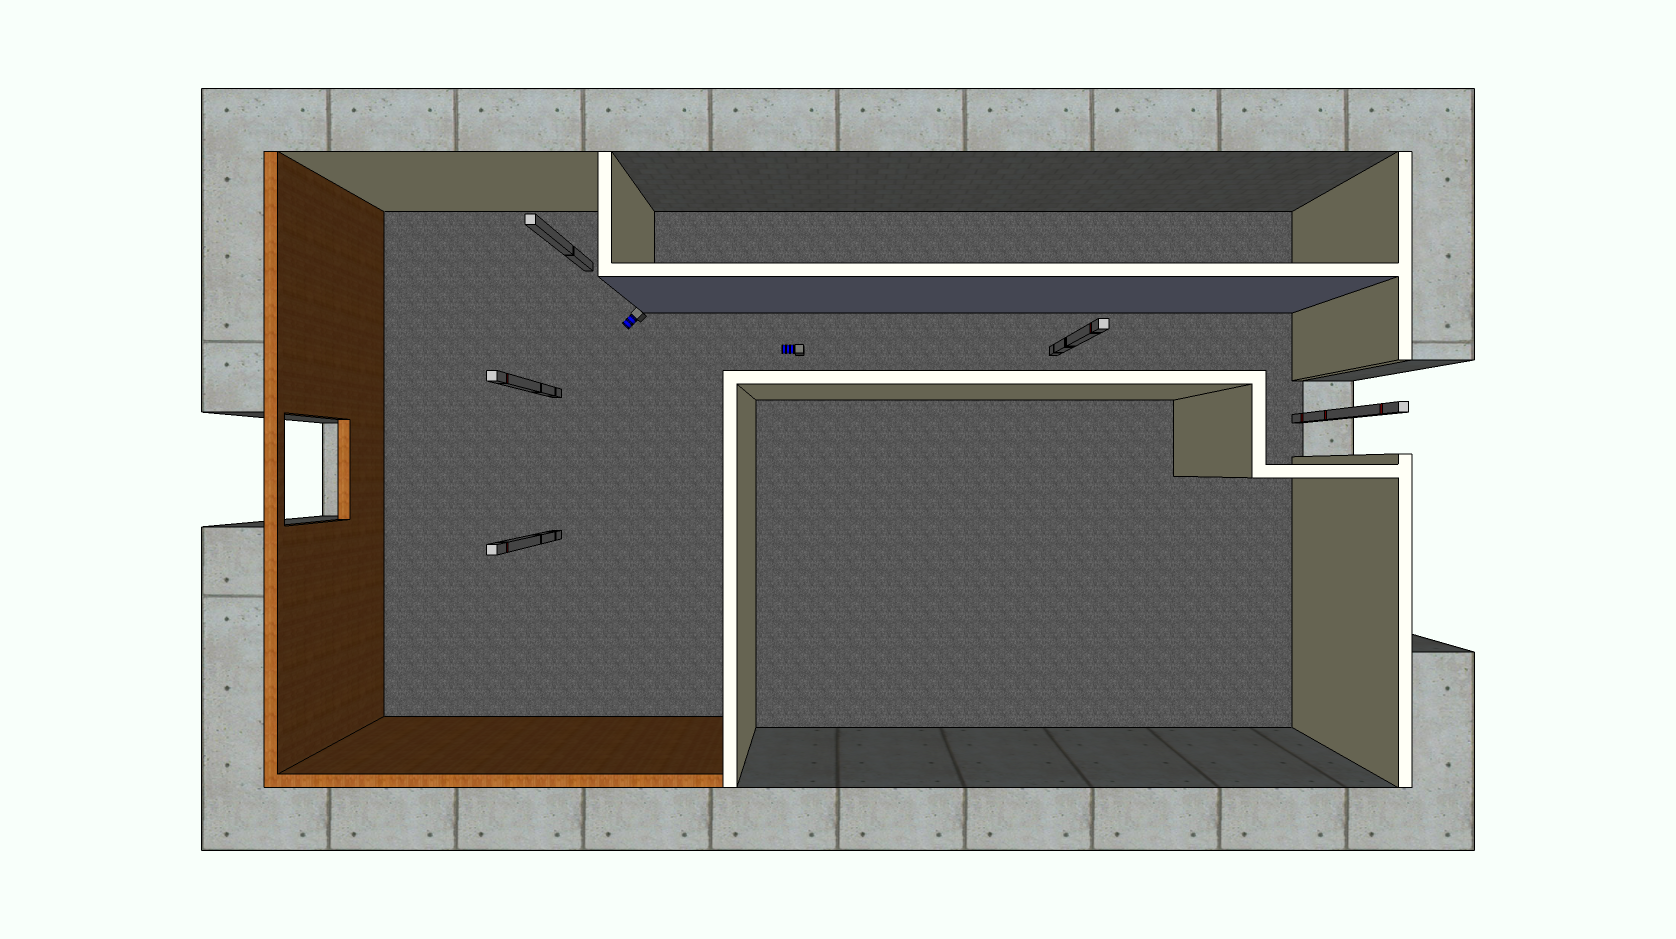
\includegraphics[width=6in]{../Figures/Pictures/DelCoSingleStory}
% 	\caption{Delaware County, PA Fire Test Structure}
% 	\label{fig:DelCoSingleStory}
% \end{figure}

\begin{figure}[!ht]
	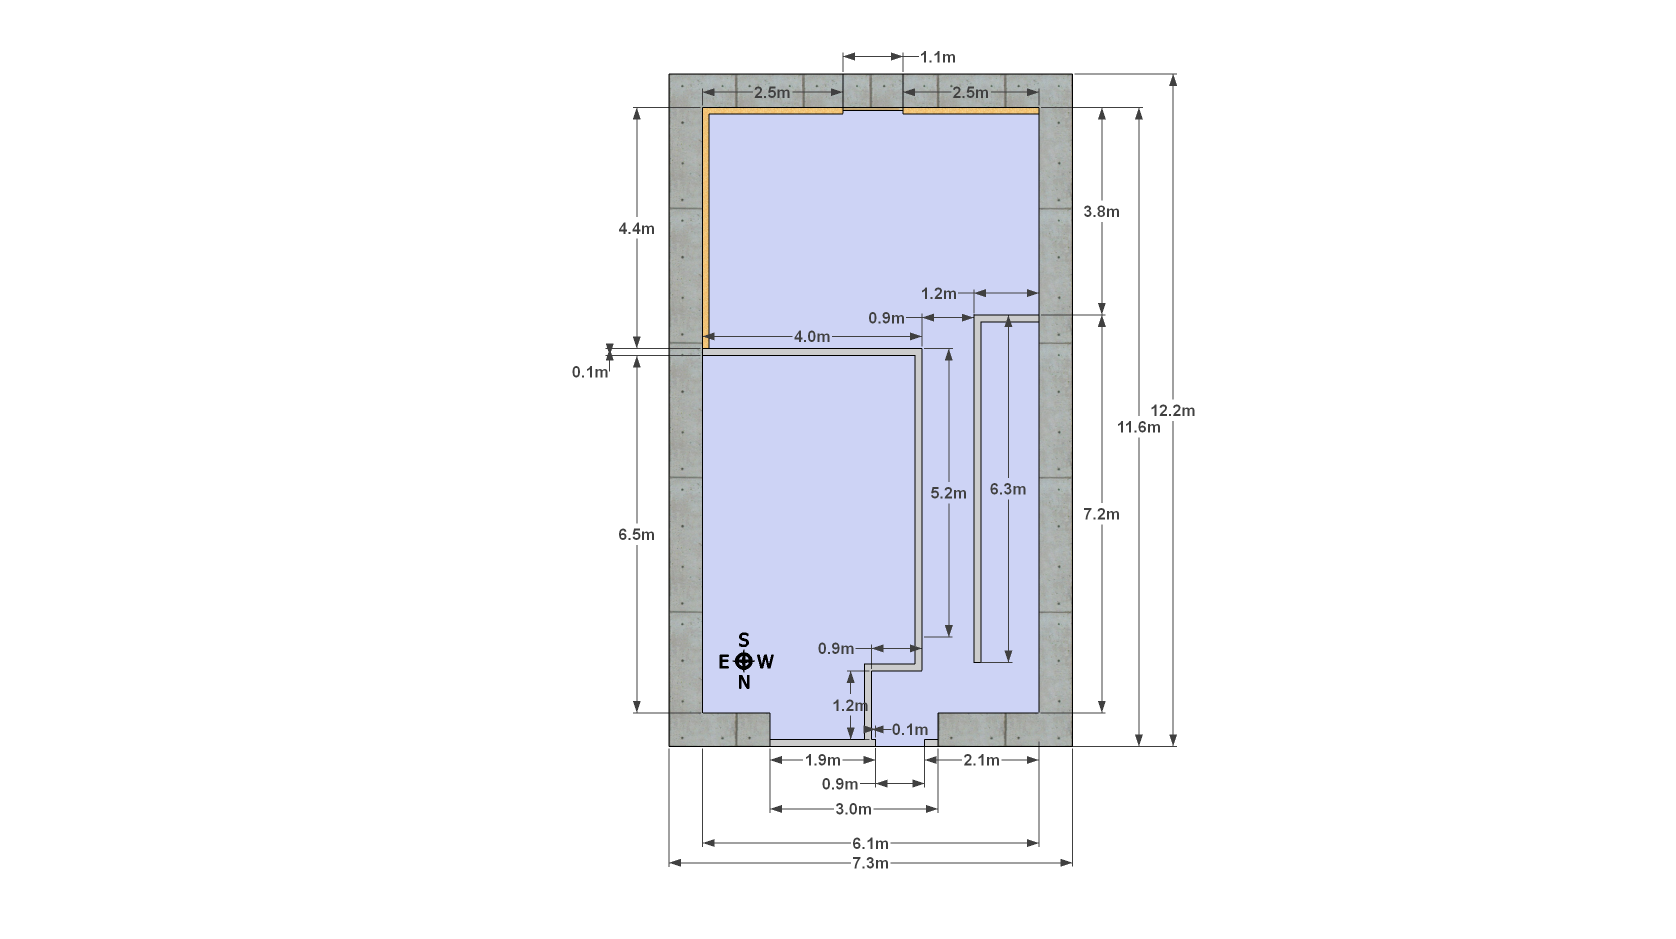
\includegraphics[width=6in]{../Figures/Pictures/DelCoSingleStoryDimensionsMetric}
	\caption{Floor Plan of the Test Structure.}
	\label{fig:Test_Structure_Floor_Plan}
\end{figure}

The floor of the structure was the concrete pad. The interior walls of the structure were framed with steel studs and track.  The studs were set to 0.40~m (16~in) centers. The ceiling support was composed of wood truss joist I-beams (TJIs) with a 299~mm (11.75~in) depth. The TJI was composed of laminated veneer lumber flanges with a cross section of 29~mm (1.125~in) x 44~mm (1.75~in) and an 11~mm (0.43~in) thick oriented strand board web. Tongue and grove, 18.3~mm (0.72~in) thick, oriented strand board was attached to the top of the TJIs.

The interior walls of the burn room were lined with 13~mm (0.5~in) thick cement board. The ceiling of the burn room was the exposed ``floor assembly". The walls of the hallway and entry foyer were composed of 16~mm (0.625~in) Type X gypsum board. The ceiling of the hallway and entry foyer was composed of two layers of 13~mm (0.5~in) thick cement board.

\clearpage

\section{Instrumentation}
\label{sec:Instrumentation}

The structures were instrumented for temperature, gas velocity, and heat flux measurements. Gas temperatures in the burn rooms were measured with bare-bead, Chromel-Alumel (type K) thermocouples. Additional single thermocouples were installed in conjunction with the bi-directional probes for gas velocity measurements. The single thermocouples were bare-bead, Chromel-Alumel (type K) thermocouples, with a 1.0~mm (0.04~in) nominal diameter. The thermocouple wire was protected with an 3.2~mm (0.125~in) diameter inconnel sheath. Schmidt-Boelter gauges were used to measure both total heat flux and radiant heat flux (radiometer). A radiometer is a total heat flux gauge with a zirconium plate to prevent contributions from convective heat transfer. A legend, which clarifies the instrumentation schematics discussed in the follow sections, is included in Fig.~\ref{fig:Instrumentation_Legend}.

\begin{figure}[!ht]
	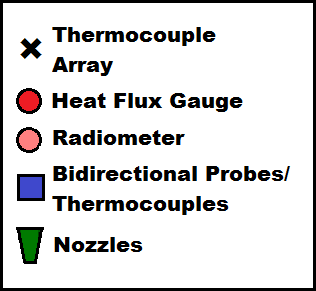
\includegraphics[width=.35\columnwidth]{../Figures/Pictures/Legend2}
	\caption{Instrumentation Legend.}
	\label{fig:Instrumentation_Legend}
\end{figure}

\subsection{Gas Cooling}
\label{subsec:Gas_Cooling_Instrumentation}

The gas cooling tests included 4 bare-bead thermocouple arrays  a bi-directional probe plus solid thermocouple array, and a total heat flux gauge/radiometer pair. Figure~\ref{fig:Gas_Cooling_Instrumentation_Dimensions} provides the positions within the burn room and gas cooling room where the senors were located (cf. Fig.~\ref{fig:Instrumentation_Legend} for reference on the symbols). Each of the bare-bead thermocouple array had 11 thermocouples. The top thermocouple was placed at the ceiling and each subsequent thermocouple was spaced 0.3~m (1~ft) apart with the bottom thermocouple being 3.05~m (10ft) below the ceiling. There were 6 velocity probes and solid thermocouples centered at the external doorway to the gas cooling room. The top probes were 0.15~m (0.5~ft) below the door soffit, the second probes were 0.3~m (1~ft), and the remaining 4 were spaced 0.3~m (1~ft) apart with the bottom probe being 1.52~m (5~ft) below the soffit. The total heat flux guage/radiometer were set to be 0.15~m (0.5~ft) off the ground and aimed to view the ceiling.

\begin{figure}[!ht]
	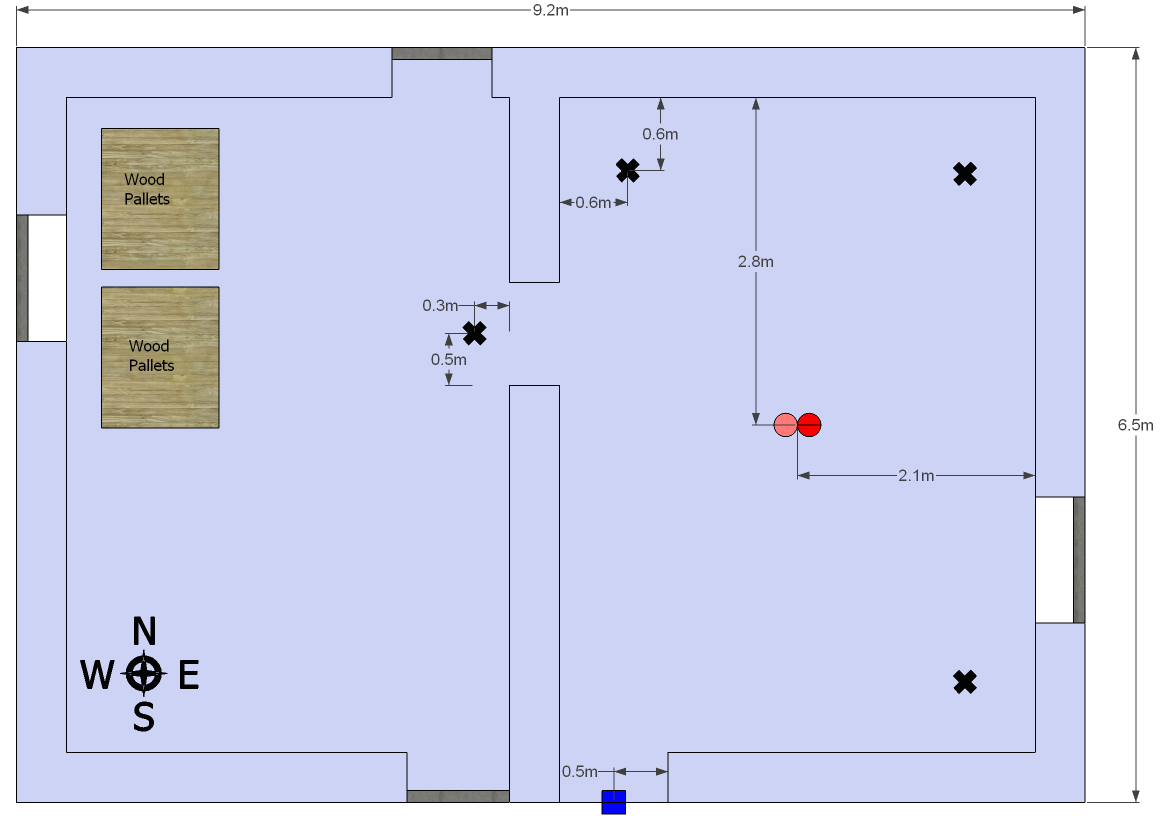
\includegraphics[width=.8\columnwidth]{../Figures/Pictures/DelCoBurnBuildingInstrumentation}
	\caption{Instrumentation Schematic for the Gas Cooling Experiments.}
	\label{fig:Gas_Cooling_Instrumentation_Dimensions}
\end{figure}

\clearpage

\subsection{Fire Suppression}
\label{subsec:Fire_Suppression_Instrumentation}

The fire suppression testing included 2 bare-bead thermocouple arrays, three bi-directional probe plus solid thermocouple arrays, 2 total heat flux gauge pairs, and 2 total heat flux guage/radiometer pairs. Figure~\ref{fig:Fire_Suppression_Instrumentation_Dimensions} provides the positions within the burn room, hallway, and entrance foyer where the senors were located (cf. Fig.~\ref{fig:Instrumentation_Legend} for reference on the symbols). Each bare-bead thermocouple array had 8 thermocouples. The top sensor was 0.03~m (1~in) below the ceiling and the remaining thermocouples were space 0.3~m (1~ft) apart with the bottom thermocouple being 2.13~m (7~ft) below the ceiling. The three bi-directional probe arrays had unique sensor locations. For the window array there were four sensor pairs located 0.28~m (0.95~ft), 0.58~m (1.90~ft), 0.84~m (2.85~ft), and 1.16~m (3.8~ft) below the soffit. For the hallway array, the 7 sensor pairs started 0.3~m (1~ft) below the ceiling and were spaced every 0.3~m (1~ft) ending 2.13~m (7~ft) below the ceiling. The doorway array also had 7 sensor pairs, but the first sensors were located 0.15~m (0.5~ft) below the soffit. The remaining sensors were spaced every 0.3~m (1~ft) with the bottom pair 1.83~m (6~ft) below the doorway soffit. The total heat flux guage/radiometer pairs were set to be 0.15~m (0.5~ft) off the ground and aimed to view the ceiling. The pairs of total heat flux guages were set 1~m (3~ft) off the ground with one sense ``looking'' vertical and the other horizontal.

\begin{figure}[!ht]
	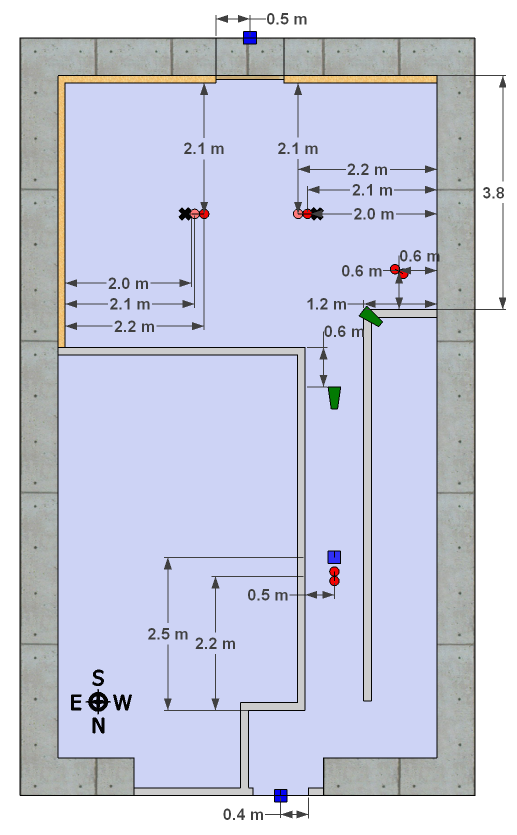
\includegraphics[width=.8\columnwidth]{../Figures/Pictures/DelCoSingleStoryInstrumentationDimensions}
	\caption{Instrumentation Schematic for the Fire Suppression Experiments.}
	\label{fig:Fire_Suppression_Instrumentation_Dimensions}
\end{figure}

\clearpage

\subsection{Measurement Uncertainty}
\label{subsec:Uncertainty}

There are different components of uncertainty in the length, mass, temperature, heat flux, gas concentration, differential pressure, gas velocity and heat release rate reported here. Uncertainties are grouped into two categories according to the method used to estimate them. Type A uncertainties are those which are evaluated by statistical methods, and Type B are those which are evaluated by other means~\cite{Taylor&Kuyatt:1994}. Type B analysis of systematic uncertainties involves estimating the upper (+ a) and lower (- a) limits for the quantity in question such that the probability that the value would be in the interval ($\pm$ a) is essentially 100~\%. After estimating uncertainties by either Type A or B analysis, the uncertainties are combined in quadrature to yield the combined standard uncertainty. Then the combined standard uncertainty is multiplied by a coverage factor of two, which results in the expanded uncertainty with a 95~\% confidence interval (2$\sigma$).  For some of these components, such as the zero and calibration elements, uncertainties are derived from referenced instrument specifications. For other components, referenced research results and past experience with the instruments provided input in the uncertainty determination.

Each length measurement was taken carefully. Length measurements such as the room dimensions, instrumentation array locations and fire apparatus (for example nozzle, sprinkler, or fan) placement were made with a hand held laser measurement device which is has an accuracy of $\pm$ 6.0 mm (0.25) over a range of 0.61 m (2.00 ft) to 15.3 m (50.0 ft)~\cite{StanleyTools}.  However, conditions affecting the measurement, such as levelness of the device, yields an estimated uncertainty of $\pm$ 0.5~\% for measurements in the 2.0~m (6.6~ft) to 10.0~m (32.8~ft) range.  Steel measuring tapes with a resolution of  $\pm$ 0.5~mm (0.02~in) were used to locate individual sensors within a measurement array and to measure and position the furniture. The steel measuring tapes were manufactured in compliance with NIST Manual 44, which specifies a tolerance of $\pm$1.6~mm (0.06~in) for 9.1~m (30~ft) tapes and $\pm$ 6.4~mm (0.25~in) for 30.5~m (100~ft) tapes~\cite{Butcher:2012}. Some issues, such as ``soft'' edges on the upholstered furniture, result in an estimated total expanded uncertainty of $\pm$ 1.0~\%.

The load cell used to weigh the fuels prior to the experiments had a range of 0~kg (0~lb) to 200~kg (440~lb) with a resolution of a 0.05~kg (0.11~lb) and a calibration uncertainty within 1~\%~\cite{Ohaus:2000}. The expanded uncertainty is estimated to be less than $\pm$ 5~\%.

The standard uncertainty in temperature of the thermocouple wire itself is $\pm$ 2.2 $^{\circ}$C at 277 $^{\circ}$C and increases to $\pm$ 9.5~$^{\circ}$C at 871~$^{\circ}$C as determined by the wire manufacturer\cite{Omega:2004}. The variation of the temperature in the environment surrounding the thermocouple is known to be much greater than that of the wire uncertainty~\cite{Blevins:1999,Pitts:2003}. Small diameter thermocouples were used to limit the impact of radiative heating and cooling. The estimated total expanded uncertainty for temperature in these experiments is $\pm$ 15~\%.

In this study, total heat flux measurements were made with water-cooled Schimidt-Bolter gauges. The manufacturer reports a $\pm$ 3~\% calibration expanded uncertainty for these devices~\cite{Medtherm:2003}. Results from an international study on total heat flux gauge calibration and response demonstrated that the uncertainty of a Schmidt-Boelter gauge is typically $\pm$ 8~\%~\cite{Pitts:2006}.

The gas measurement instruments and sampling system used in this series of experiments have been demonstrated an expanded (k = 2) relative uncertainty of $\pm$ 1~\% when compared with span gas volume fractions~\cite{Bundy:2007}. Given the non-uniformities and movement of the fire gas environment and the limited set of sampling points in these experiments an estimated uncertainty of $\pm$ 12~\% is being applied to the results~\cite{Lock:1}.

Differential pressure reading uncertainty components were derived from pressure transducer instrument specifications and previous experience with pressure transducers. The transducers were factory calibrated and the zero and span of each was checked in the laboratory prior to the experiments yielding an accuracy of $\pm$ 1~\%~\cite{Setra:2002}. The total expanded uncertainty was estimated at 10~\%.

Bi-directional probes and single thermocouples were used to measure the velocity.  The bi-directional probes used similar pressure transducers as those used for the differential pressure measurements discussed above. Bare-bead Type K thermocouple are co-located with the probe. A gas velocity measurement study, examining the doorway flow of pre-flashover compartment fires, yielded expanded uncertainty measurements ranging from $\pm$ 0.14 to $\pm$ 0.22 for bi-directional probes of similar design~\cite{Bryant:FSJ2009}. The total expanded uncertainty for gas velocity in these experiments w estimated to be  $\pm$ 18~\%.

Water flowrate was measured with a pressure and flow meter combination. The meter consists of a section of 6.35~cm (2.5~inch) cast aluminum pipe with a 0 - 4.1~MPa (0 - 600~psi) pressure transducer and a paddlewheel type flow sensor with a range of 0 to 4800~lpm (1250~gpm). The pressure transducer and paddlewheel both connect to the battery operated control box where the pressure transducer voltage is converted to a pressure and the paddlewheel pulse count is converted to a volumetric flow rate.  The manufacturer reports a $\pm$ 5~\% calibration expanded uncertainty for the flow sensor and $\pm$ 3~\%  for the pressure sensor~\cite{Akron:2009}. The pressure transducer was calibrated with a known analog pressure gauge. The flow meter was calibrated by capturing water over time and measuring that mass of water to determine the flowrate. The total expanded uncertainty was estimated at $\pm$ 10~\%.

\section{Fuel Load}
\label{sec:fuel_load}

\subsection{Gas Cooling}
\label{sec:Fuel_Load_Gas_Cooling}

Wood pallets were used as the fuel source for the gas cooling experiments. The pallets were approximately 1.2~m (4.0~ft) by 1.0~m (3.3~ft) by 0.13~m (0.42~ft) thick. The pallets ranged in mass from 13.6~kg (29.9~lb) to 26.4~kg (58.1~lb) with an average of 18.4~kg (40.5~lbs). The initial fuel load consisted of 10 pallets, arranged in two stacks of five as shown in Fig.~\ref{fig:Burn_Building_Fuel_Load}. Approximately one half of a bale of excelsior, 13.0~kg (28.6~lb), was mixed with the pallets to aid with ignition. Fig.~\ref{fig:Burn_Building_Fuel_Load}, also provides dimensioned locations of the two stacks of pallets within the burn room.

\begin{figure}[!ht]
	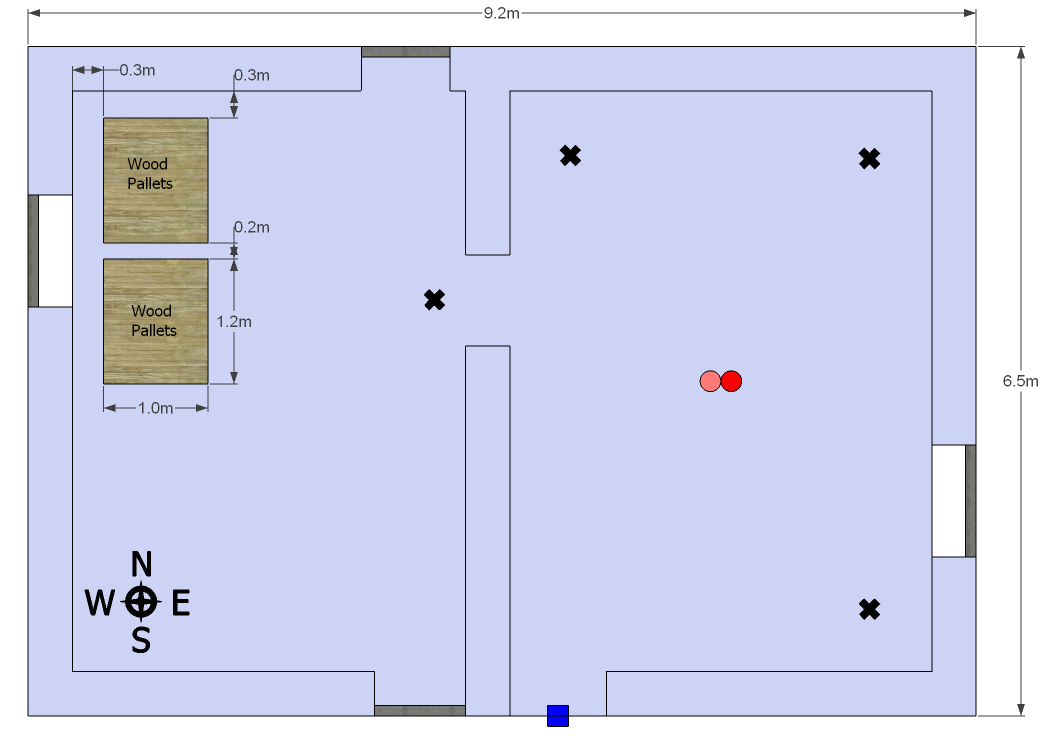
\includegraphics[width=6in]{../Figures/Pictures/DelCoBurnBuildingFuelLoad}
	\caption{Burn Building Fuel Load.}
	\label{fig:Burn_Building_Fuel_Load}
\end{figure}

Note, that as the pallets burned away and the hot gas layer temperatures decreased, the steel shutters on the window to the burn room were opened and additional pallets were added. Pallets were added to the existing fuel locations until the flames from the piles reached the ceiling of the burn room again. The number of pallets added each time varied.

\clearpage

\subsection{Fire Suppression}
\label{sec:Fuel_Load_Fire_Suppression}

\subsubsection{Wood Fuel Package}
\label{sec:fire_suppression_pallet_fuel}

The fuel load for these experiments consisted of one bale of hay, twelve pallets, eleven and a half sheets plywood on the walls and the wood ``floor assembly". Two stacks of pallets with hay were used as the first items ignited in each experiment. Each stack was composed of six pallets with a half bale of hay. The hay was layered between each pallet. Figure~\ref{fig:Wood_Fuel_Load} shows the pallets prior to ignition. The pallets and hay were weighed prior to each experiment. For the four pallet experiments, the average mass of the two stacks of pallets and the bale of hay was 232.4~kg (511.3~lb). A complete listing of the mass of each pallet and hay bales is given in Appendix~\ref{app:fuel_loads}.

\begin{figure}[!ht]
	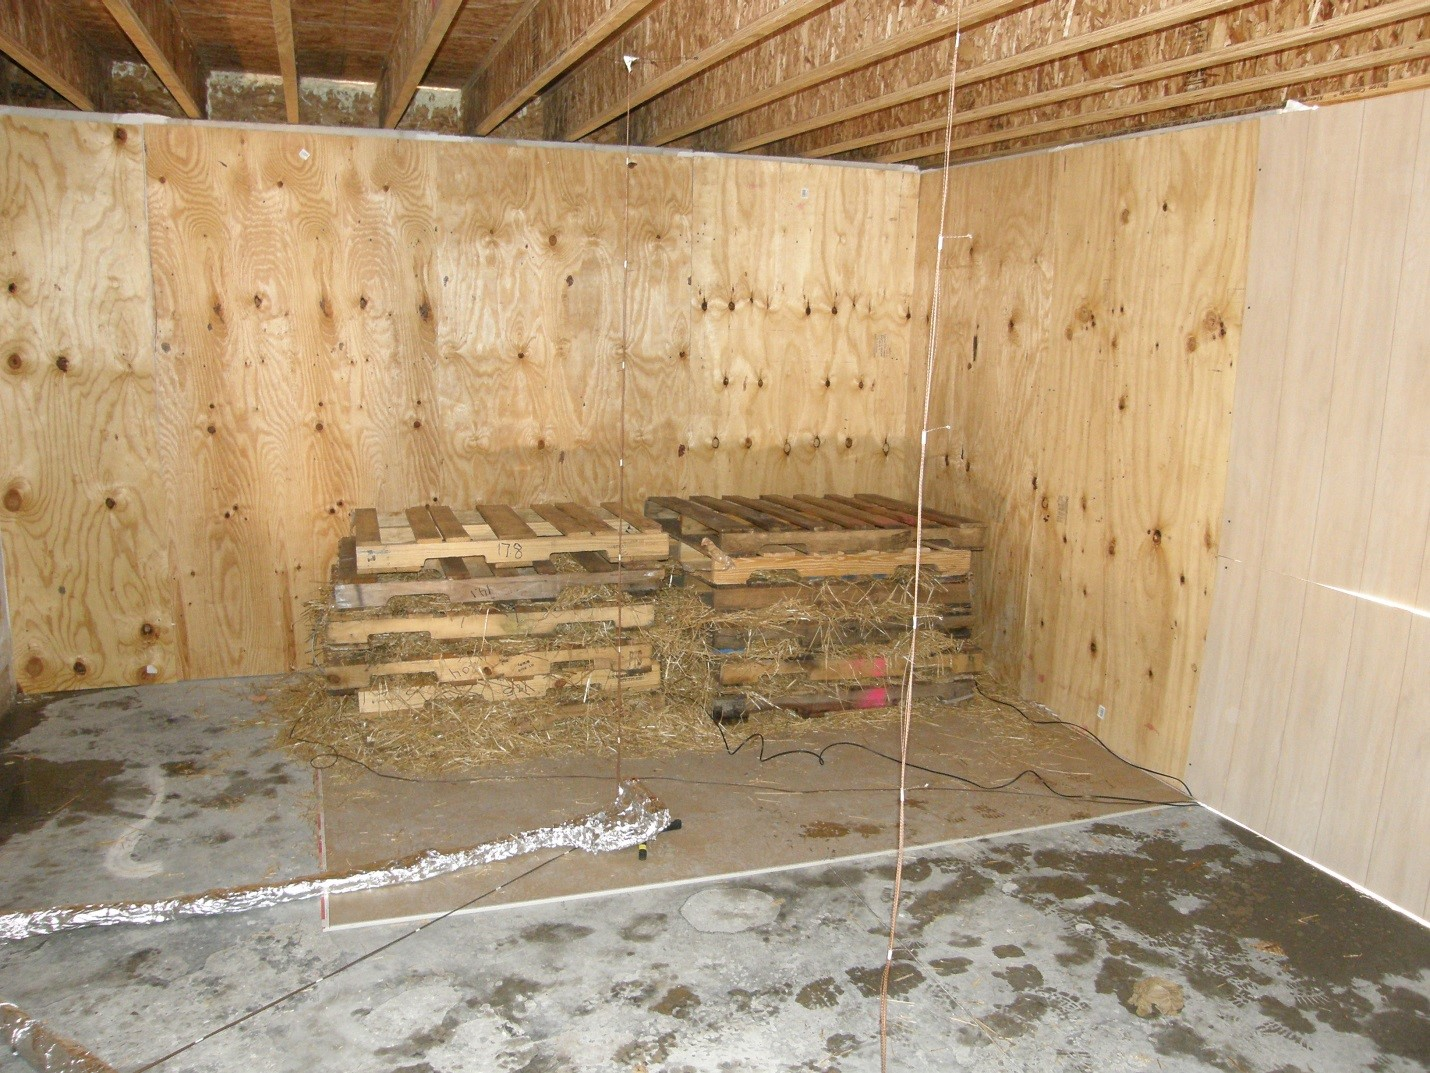
\includegraphics[width=0.65\columnwidth]{../Figures/Pictures/Wood_Fuel_Package}
	\caption{Photograph of Southeast corner of burn room with wood fuel load.}
	\label{fig:Wood_Fuel_Load}
\end{figure}

The pallet stacks were located 0.3~m (12~in) away from the east and south walls of the burn room (cf. Fig.~\ref{fig:Wood_Fuel_Load_Dimensions}). The pallets were 1.2~m (48~in) long, 1.0~m (40~in) and 123~mm (4.8~in) high. The stacks were spaced 150~mm (6~in) apart. One layer of 13~mm (0.5~in) thick gypsum board panels were laid on the concrete floor under the wood pallets to form a protective layer to minimize thermal damage to the concrete floor. The east and south wall of the burn room was covered with 15~mm (0.59~in) thick, sheets of plywood.  The ``wood flooring assembly", composed of 12 TGIs and 9 sheets of OSB, served as the ceiling of the burn room. The open doorway to the burn room on the south side was covered with a 2.4~m (8~ft) tall by 1.2~m (4~ft) wide piece of medium density fiberboard paneling that was 5~mm (0.19~in) thick.

\begin{figure}[!ht]
	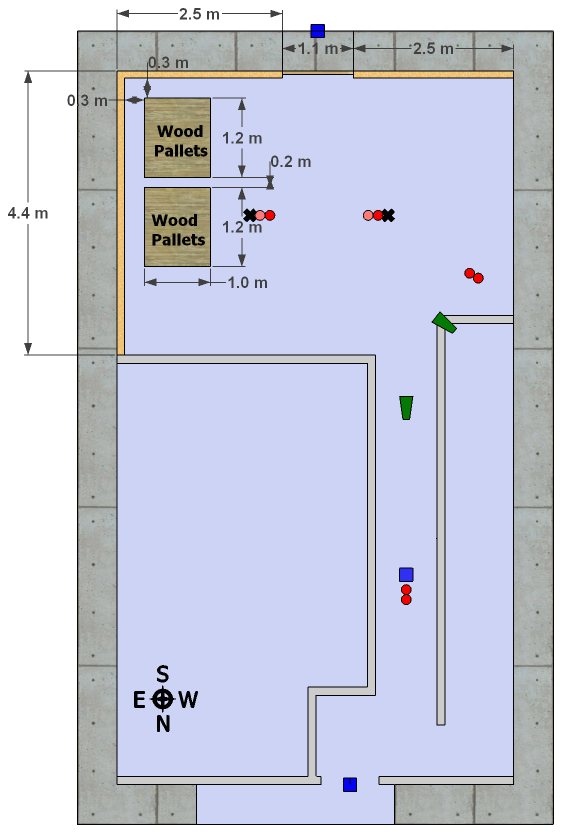
\includegraphics[width=.8\columnwidth]{../Figures/Pictures/DelCoSingleStoryWoodFuelLoad}
	\caption{Wood Fuel Load Dimensions.}
	\label{fig:Wood_Fuel_Load_Dimensions}
\end{figure}

\clearpage

\subsubsection{Furniture Fuel Package}
\label{sec:fire_suppression_furniture_fuel}

The fuel load for these experiments consisted of 2 sleeper sofas and 2 chairs, carpet, padding, and wood paneling along the southeast corner walls. An image of the fuel arrangement is shown in Fig.~\ref{fig:Furniture_Fuel_Load}. The couches and chairs are setup to mimic a typical seating area with one couch against the south and east wall respectively with each being 0.9~m (36~in) away from the corner. A chair is placed adjecent to each couch and the specific locations can be found in the dimensioned schematic, Fig.~\ref{fig:Furniture_Fuel_Load_Dimensions}. In total, this fuel package contains approximately 336 kg of fuel consisting of wood, polyurethane (PU), polyester (PET),and polyprolene (PP). Table~\ref{tab:Fire_Suppression_Fuel_Masses} provides a breakdown on the fuel composition for these experiments.

\begin{figure}[!ht]
	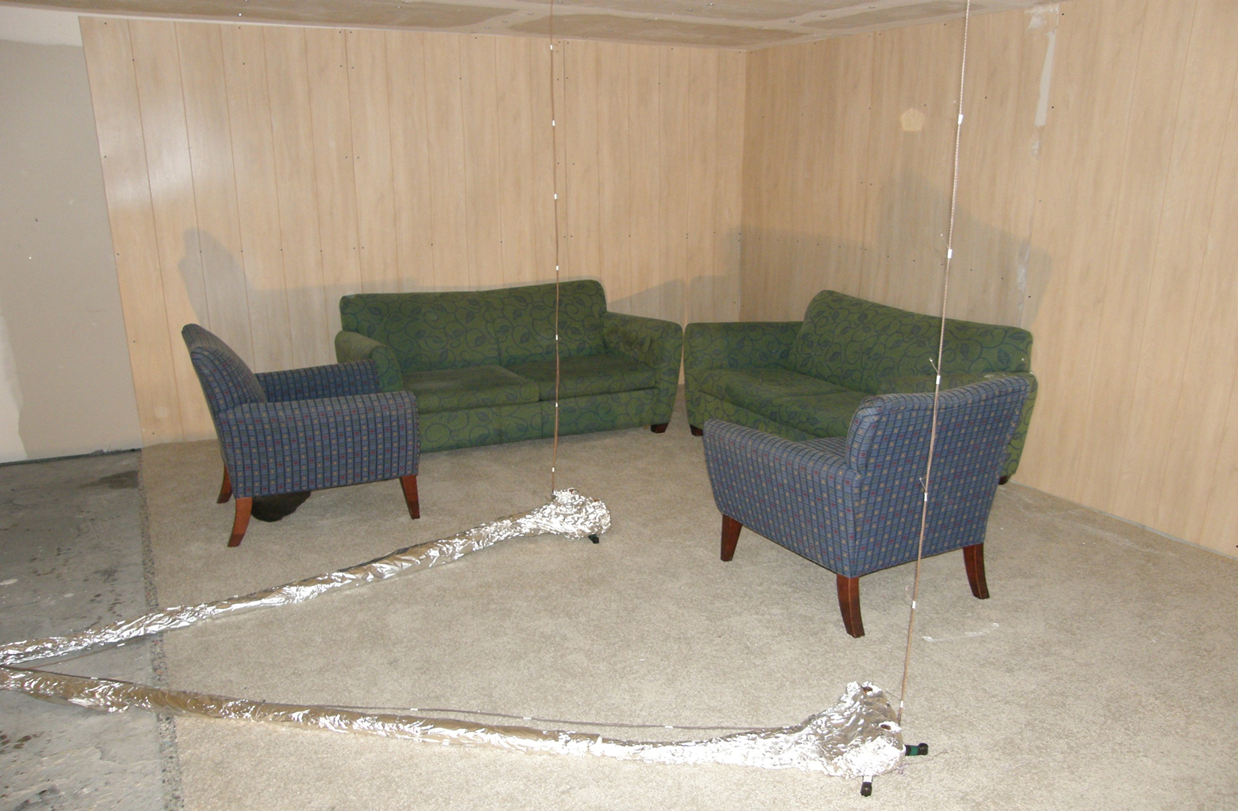
\includegraphics[width=.8\columnwidth]{../Figures/Pictures/Furniture_Fuel_Load}
	\caption{Furniture Fuel Load Dimensions.}
	\label{fig:Furniture_Fuel_Load}
\end{figure}

\begin{figure}[!ht]
	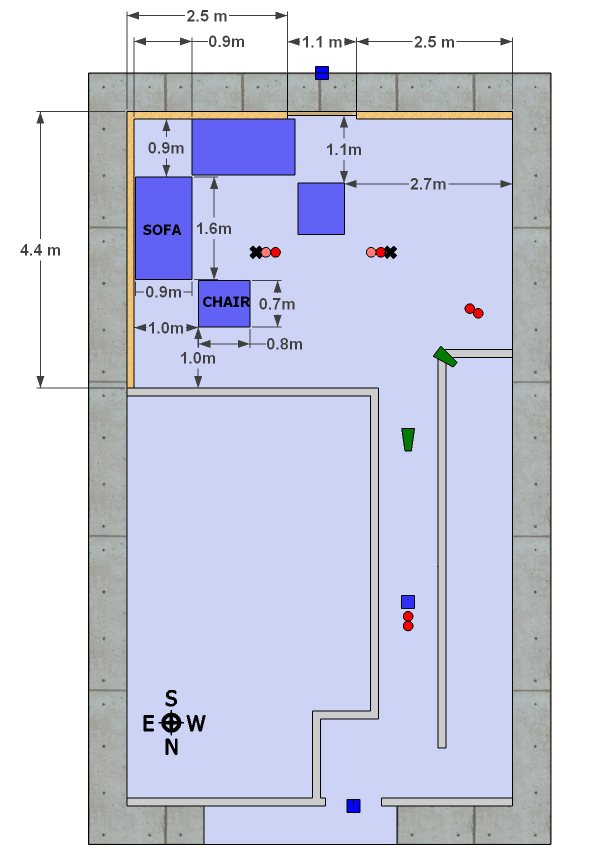
\includegraphics[width=.8\columnwidth]{../Figures/Pictures/DelCoSingleStoryFurnitureFuelLoad}
	\caption{Furniture Fuel Load Dimensions.}
	\label{fig:Furniture_Fuel_Load_Dimensions}
\end{figure}

\begin{sidewaystable}[!ht]
	\centering
	\scriptsize
	\caption{Fire Suppression Fuel masses}
	\renewcommand{\tabcolsep}{1pt}
	\begin{tabular}{lllllcc}
		\toprule[1.5pt]
		Item               & Component		& Quantity		&  Material Description             			&  Dimensions (m)            	&  Mass (kg)  		& Total Mass (kg) \\
		\midrule
		2-seat Sofa        &				& 2				& 85~\% PU Foam, 15~\% PET Fiber, Wood Frame 	&  1.68 L X 0.90 D X 0.86 H  	&  72.4    			& 144.8 \\
		           	 	   & Mattress	    & 1 per sofa	& Cover: 52~\% PP, 48~\% PET,                   &  1.83 L X 1.21 W X 0.14 H     &  14.6             & \\
		           	 	   &                &               & Filling: 66~\% PET Pad, 34~\% PET Batting     &                               &                   & \\
			           	   & Cushion    	& 2 per sofa	& 85~\% PU Foam, 15~\% PET Fiber   				&  0.69 L X 0.58 D X 0.14 H  	&  2.2     			& \\
		Blue Chair         &				& 2				& 85~\% PU Foam, 15~\% PET Fiber, Wood Frame   	&  0.81 L X 0.75 D X 0.91 H  	&  17.4    			& 34.8 \\
		    			   & Cushion        & 1 per chair   & 85~\% PU Foam, 15~\% PET Fiber				&  0.51 L X 0.57 D X 0.14 H  	&  1.7    			& \\
		Blue/Green Chair   & 				& 2				& 85~\% PU Foam, 15~\% PET Fiber, Wood Frame    &  0.77 L X 0.71 D X 0.89 H  	&  16    			& 32 \\
		                   & Cushion    	& 1 per chair	& 85~\% PU Foam, 15~\% PET Fiber		        &  0.55 L X 0.53 D X 0.15 H  	&  1.6    			& \\
		Paneling           &				& 8 panels		& Medium density fiberboard                     &  2.44 L X 1.22 W X 3.2~mm H   &  9    			& 72 \\
		Carpeting          &				& 22.3 m$^2$	& 100~\% PET                  					&  3.68 L X 6.05 W  			&  32.2				& 32.2 \\
		Carpet Padding     &				& 22.3 m$^2$	& PU                       	 				    &  3.68 L X 6.05 W X 11~mm H    &  19.8			    & 19.8 \\
		                   &                &               &                                               &                               & Total Mass        & 335.6 \\
		\bottomrule[1.25pt]
	\end{tabular}
	\label{tab:Fire_Suppression_Fuel_Masses}
\end{sidewaystable}

\chapter{Experiments and Results}
\label{chap:Experiments_and_Results}

\section{Spray Density}
\label{sec:Spray_Density}

Spray density experiments were conducted by placing 0.23~m$^2$ (2.5~ft$^2$) interlocking collector bins across the floor surface area of the burn rooms within each structure. The buildings were sheathed in plastic for the spray density tests to protect and preserve as much of the structure as possible before any fire suppression tests were conducted. Water flowed for a specified duration and upon completion the bins were removed from the structure. Each bin was then weighed to quantify the impact of nozzle location and spray pattern. Thirty-three spray density tests were conducted; 21 were in the burn building and 12 were in the concrete structure. Table~\ref{tab:spray_density_tests} provides an overview of each experiment. In the table, BB stands for the burn building tests while CS stands for the concrete structure tests. For all of the experiments, 100~ft (30~m) of 1~3/4~inch hoseline connected to a Blitz Fire monitor with a Metro 1 nozzle was used.

\begin{table}[!ht]
\footnotesize
\centering
\captionof{table}{Spray Density Test Matrix}\label{tab:spray_density_tests}
\begin{tabular}{lllllll}
\toprule[1.5pt]
Test \#    &   Flow Rate (gpm)  & Duration (s)  & Fluid  &  Pattern            & Nozzle Height (in) & Location (in) \\
\midrule
BB1        &   123              & 15            & Water  &  Solid Stream back  & 20~7/8             &          \\
BB2        &   122              & 23            & Water  &  Solid Stream       &                    &          \\
BB3        &   119              &               & Water  &  Solid Stream       & 16                 &          \\
BB4        &   118              &               & Water  &  Solid Stream       & 16                 &          \\
BB5        &   118              & 20            & Water  &  Solid Stream       & 16                 &          \\
BB6        &   120              & 21            & Water  &  30$^{\circ}$ Fog   & 15                 &          \\
BB7        &   118              & 21            & Water  &  30$^{\circ}$ Fog   & 15                 &          \\
BB8        &   119              & 22            & Water  &  30$^{\circ}$ Fog   & 17                 &          \\
BB9        &   120              & 24            & Water  &  30$^{\circ}$ Fog   & 17~1/2             &          \\
BB10       &   127              & 20            & Water  &  Solid 7/8~in Slug  & 12~1/2             &          \\
BB11       &   120              & 22            & Water  &  Solid 7/8~in Slug  & 11~1/2             &          \\
BB12       &   120 / 60cfm      & 15            & CAF    &  Smooth Bore 7/8~in & 12~1/2             &          \\
BB13       &   120 / 60cfm      & 10            & CAF    &  Smooth Bore 7/8~in &                    &          \\
BB14       &   120 / 60cfm      & 15            & CAF    &  Smooth Bore 7/8~in &                    &          \\
BB15       &   120 / 60cfm      & 20            & CAF    &  Smooth Bore 7/8~in &                    &          \\
BB16       &   120 / 60cfm      &               & CAF    &  30$^{\circ}$ Fog   & 15                 &          \\
BB17       &   120 / 60cfm      & 20            & CAF    &  Solid Stream narrow & 15                &          \\
BB18       &   120 / 60cfm      & 10            & CAF    &  Solid Stream mid   &                    &          \\
BB19       &   120 / 60cfm      & 15            & CAF    &  30$^{\circ}$ Fog   & 15                 &          \\
BB20       &   120 / 60cfm      &               & CAF    &  30$^{\circ}$ Fog   & 17                 &          \\
BB21       &   120 / 60cfm      &               & CAF    &  Solid Stream back  &                    &          \\
CS1        &   115              & 7             & Water  &  Solid Stream       &                    &          \\
CS2        &   115              & 18            & Water  &  Solid Stream       &                    &          \\
CS3        &   120              & 19            & Water  &  Solid Stream       &                    &          \\
CS4        &   118              & 21            & Water  &  Solid Stream       &                    &          \\
CS5        &   118              & 22            & Water  &  30$^{\circ}$ Fog   &                    &          \\
CS6        &   118              & 19            & Water  &  30$^{\circ}$ Fog   &                    &          \\
CS7        &   125              & 16            & Water  &  Solid 7/8~in Slug  &                    &          \\
CS7.2      &   120              & 17            & Water  &  Solid 7/8~in Slug  & 18                 &          \\
CS8        &   116              & 15            & Water  &  30$^{\circ}$ Fog   &                    &          \\
CS9        &   116              & 16            & Water  &  30$^{\circ}$ Fog   &                    &          \\
CS10       &   116              & 16            & Water  &  Solid Stream       &                    &          \\
CS11       &   117              & 16            & Water  &  Solid Stream       &                    &          \\
\bottomrule[1.25pt]
\end{tabular}\par
\end{table}

\clearpage

After weighing each of the bins the mass of water (kg) in each bin was plotted by position to visualize the spray distribution. Figure~\ref{fig:Burn_Building_Test_1} shows that with a straight stream positioned {\bf here} the majority of the water accumulated along the north and east walls of the gas cooling room within the burn building (cf. Fig.~\ref{fig:Delaware_County,_PA_Burn_Building_Layout}). Figure~\ref{fig:Burn_Building_Test_7} shows difference a fog stream as the distribution of water is far more dispersed around the gas cooling room. The remainder of the burn building spray density figures are included in Appnedix~\ref{app:spray_density}.

\begin{figure}[!ht]
	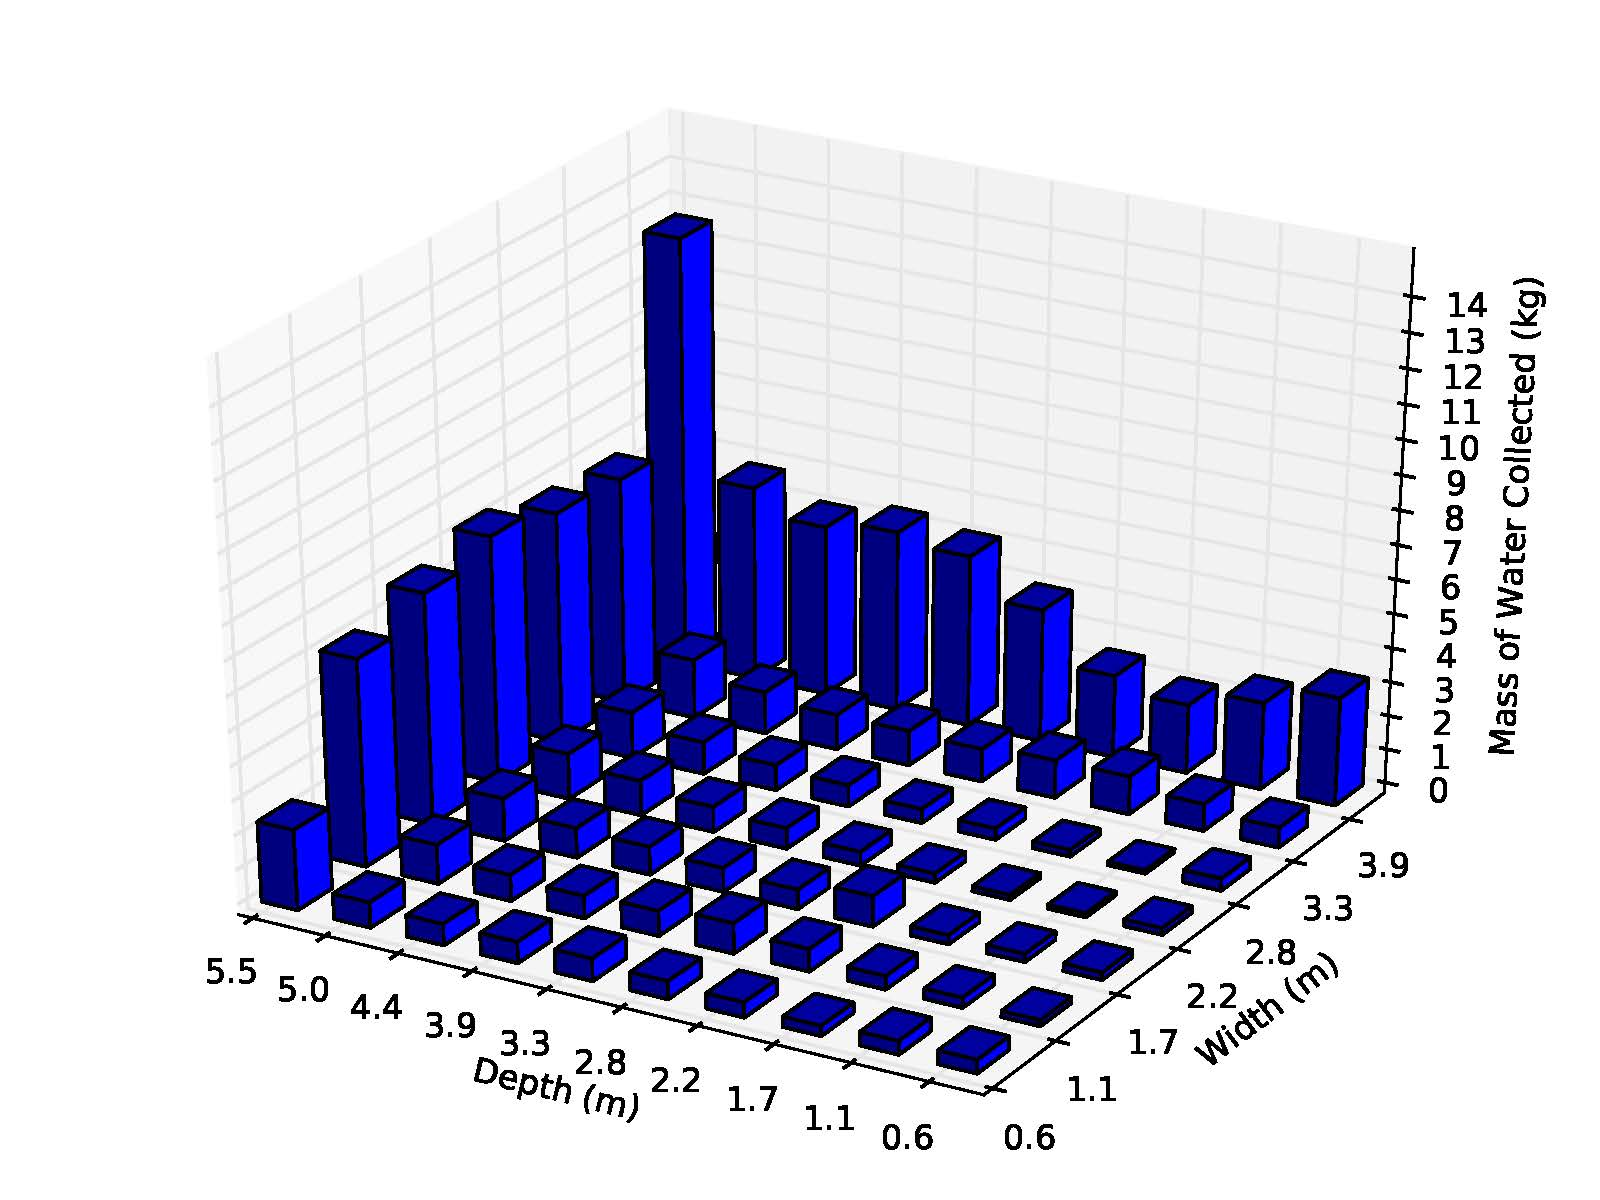
\includegraphics[width=4in]{../Figures/Bars/BB1}
	\caption{Burn Building Test 1}
	\label{fig:Burn_Building_Test_1}
\end{figure}

\begin{figure}[!ht]
	\includegraphics[width=4in]{../Figures/Bars/BB7}
	\caption{Burn Building Test 7}
	\label{fig:Burn_Building_Test_7}
\end{figure}


\clearpage

\section{Gas Cooling}
\label{sec:Gas_Cooling}

\section{Fire Suppression}
\label{sec:Fire_Suppression}
There were 14 suppression tests conducted in the single story purpose-built concrete structure. Four of the tests used a wood pallet fuel load (Section~\ref{sec:fire_suppression_pallet_fuel}) and the remaining tests used a fuel load comprised of typical household furnishings that included wooden wall paneling, two sofas, two overstuffed chairs, carpet, and padding (Section~\ref{sec:fire_suppression_furniture_fuel}). Ignition occurred in the rear of the single story structures and the available ventilation was both through the front doorway. For several tests a rear window was opened to provide additional ventilation (see Table~\ref{tab:Test_Descriptions}). The fires were intended to replicate room and contents fires typically seen within residential structures. Hose lines were pre-deployed with fixed nozzles set in two locations: one in the hallway on the approach to the burn room (hallway nozzle) and one just inside the burn room to the right side of the hallway (room nozzle). Each nozzle flowed 15~s of water or compressed air foam depending on the test. The hallway nozzle was intended to simulate a crew advancing into a structure towards the burn room. Suppression from this location would be in the form of gas cooling as the stream was not aimed at the seat of the fire (indirect interior attack). The room nozzle was intended to simulate a crew which had advanced into a structure, entered the fire room, positioned just to the side of the entry door, and began suppression on the seat of the fire (direct interior attack). Table~\ref{tab:Test_Descriptions} provides an overview of the suppression tests conducted.

\begin{table}[!ht]
	\centering
	\caption{Fire Suppression Test Descriptions}
	\begin{tabular}{llllll}
		\hline\noalign{\smallskip}
		Test		& Agent		& Stream				& Flow Rate			& Fuel           & Ventilation     \\
		\noalign{\smallskip}\hline\noalign{\smallskip}
		1 (FSE1)    &  CAF      &  30$^{\circ}$ Fog  	&  120~gpm/60~cfm   & Furniture      & Door            \\
		2 (FSW2)   	&  Water    &  30$^{\circ}$ Fog  	&  120~gpm    		& Furniture      & Door            \\
		3 (FSW3) 	&  CAF      &  7/8" Smooth Bore  	&  120~gpm/60~cfm   & Furniture      & Door            \\
		4 (FSE4)    &  Water    &  7/8" Smooth Bore  	&  120~gpm    		& Furniture      & Door            \\
		5 (FSE5)    &  Water    &  30$^{\circ}$ Fog  	&  120~gpm    		& Furniture      & Door + Window   \\
		6 (FSW6)    &  CAF      &  30$^{\circ}$ Fog  	&  120~gpm/60~cfm   & Furniture      & Door + Window   \\
		7 (FSW7)    &  Water    &  30$^{\circ}$ Fog  	&  120~gpm    		& Furniture      & Door + Window   \\
		8 (FSE8)    &  CAF      &  30$^{\circ}$ Fog  	&  120~gpm/60~cfm   & Furniture      & Door + Window   \\
		9 (Attic 1) &  Water    &  Straight Stream  	&  120~gpm    		& Furniture      & Door            \\
		10 (Attic 2)&  CAF      &  Straight Stream  	&  120~gpm/60~cfm   & Furniture      & Door            \\
		11 (FSE11)  &  Water    &  30$^{\circ}$ Fog  	&  120~gpm   		& Wood           & Door + Window   \\
		12 (FSW12)  &  CAF      &  30$^{\circ}$ Fog  	&  120~gpm/60~cfm   & Wood           & Door + Window   \\
		13 (FSE13)  &  Water    &  30$^{\circ}$ Fog  	&  120~gpm    		& Wood           & Door + Window   \\
		14 (FSW14)  &  CAF      &  30$^{\circ}$ Fog  	&  120~gpm/60~cfm   & Wood           & Door + Window   \\
		\noalign{\smallskip}\hline
	\end{tabular}
	\label{tab:Test_Descriptions}
\end{table}

\subsection{Furniture Fuel Package}
\label{subsec:Furniture_Fuel_Package}

Figures~\ref{fig:Test_1_First_Suppression} and \ref{fig:Test_1_Second_Suppression} provide and overview of the impact of 30$^{\circ}$ fog CAF application after 15~s of application from the hallway nozzle and then 15~s of application from the room nozzle. The figures provide change in temperature and heat flux at several positions and elevations through the structure. These values are taken immediately before and after application to assess the application agent, stream, and location on interior conditions.

\begin{figure}[!ht]
	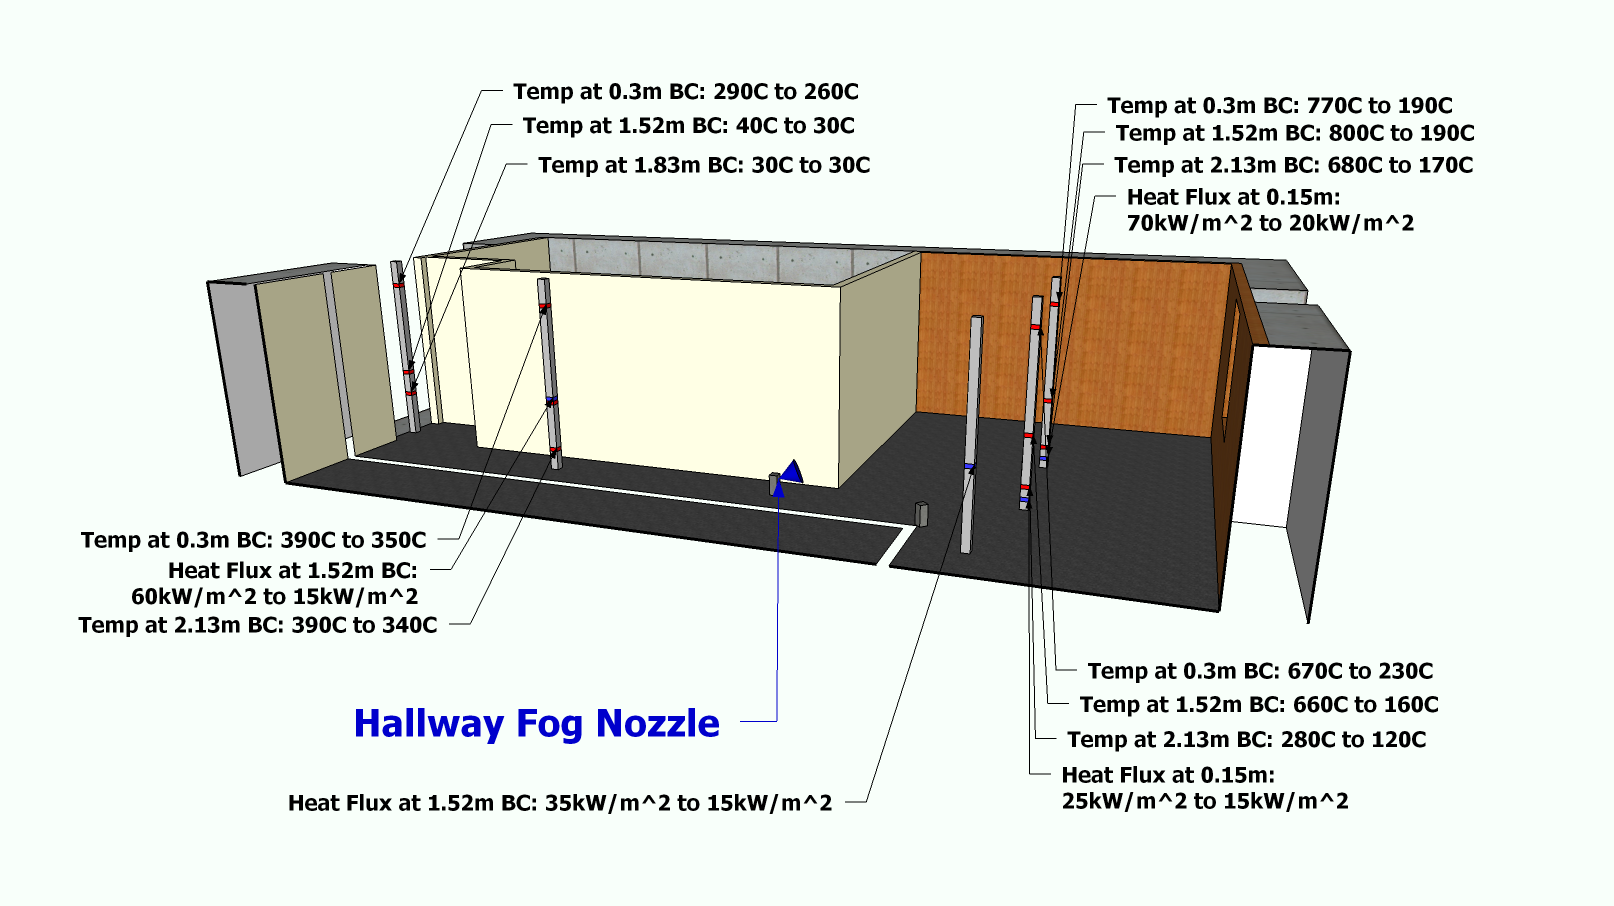
\includegraphics[width=6in]{../Figures/Pictures/Metric/DelCoFogTest1FirstSuppression}
	\caption{Test 1: Furniture Fuel Package, CAFS, 30$^{\circ}$ Fog, 120 gpm/60cfm, First Suppression}
	\label{fig:Test_1_First_Suppression}
\end{figure}

\begin{figure}[!ht]
	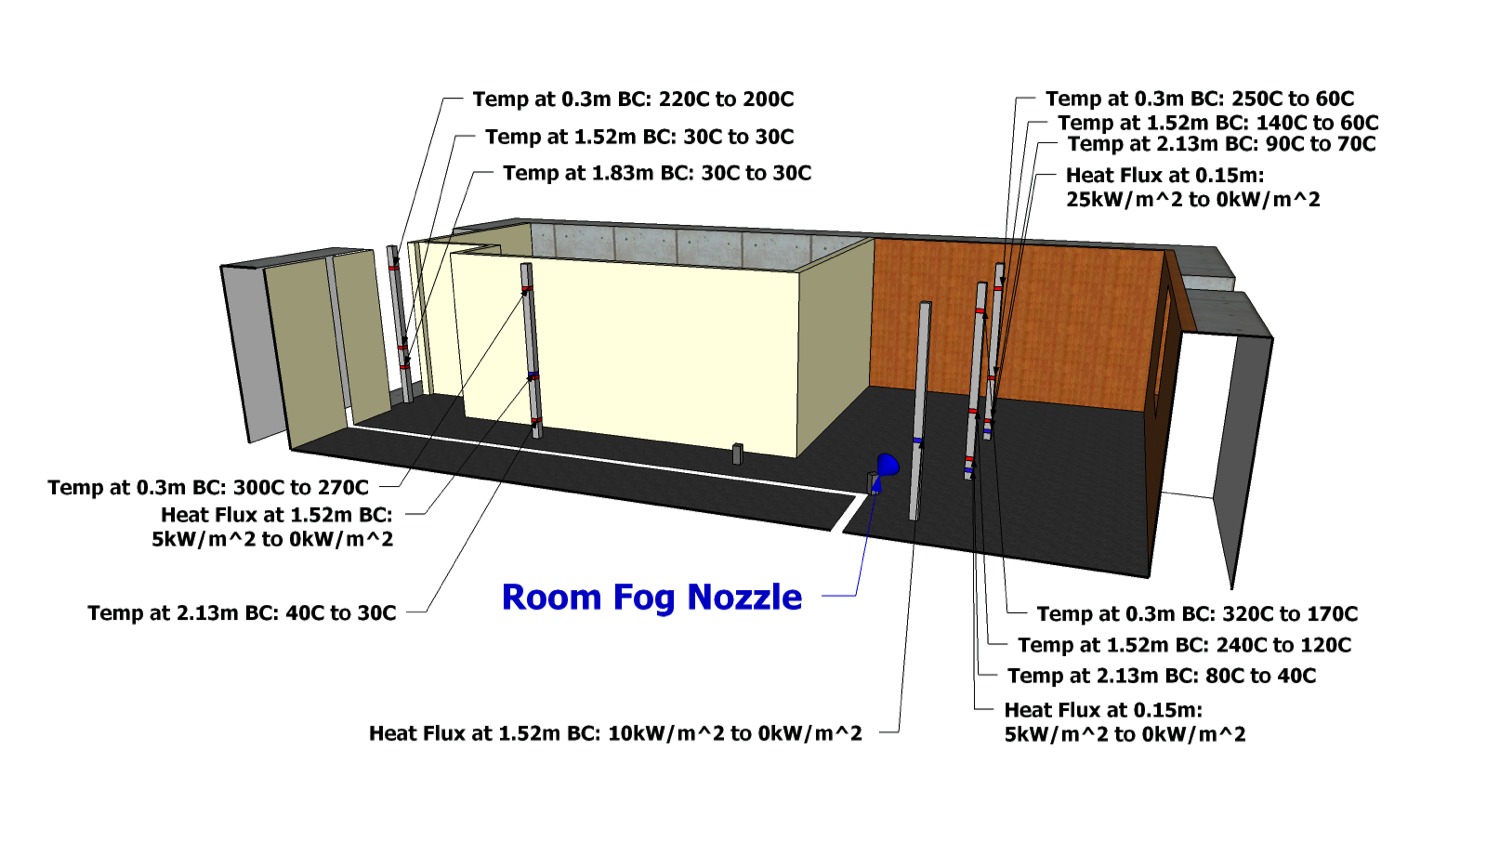
\includegraphics[width=6in]{../Figures/Pictures/Metric/DelCoFogTest1SecondSuppression}
	\caption{Test 1: Furniture Fuel Package, CAFS, 30$^{\circ}$ Fog, 120 gpm/60cfm, Second Suppression}
	\label{fig:Test_1_Second_Suppression}
\end{figure}

\begin{figure}[!ht]
	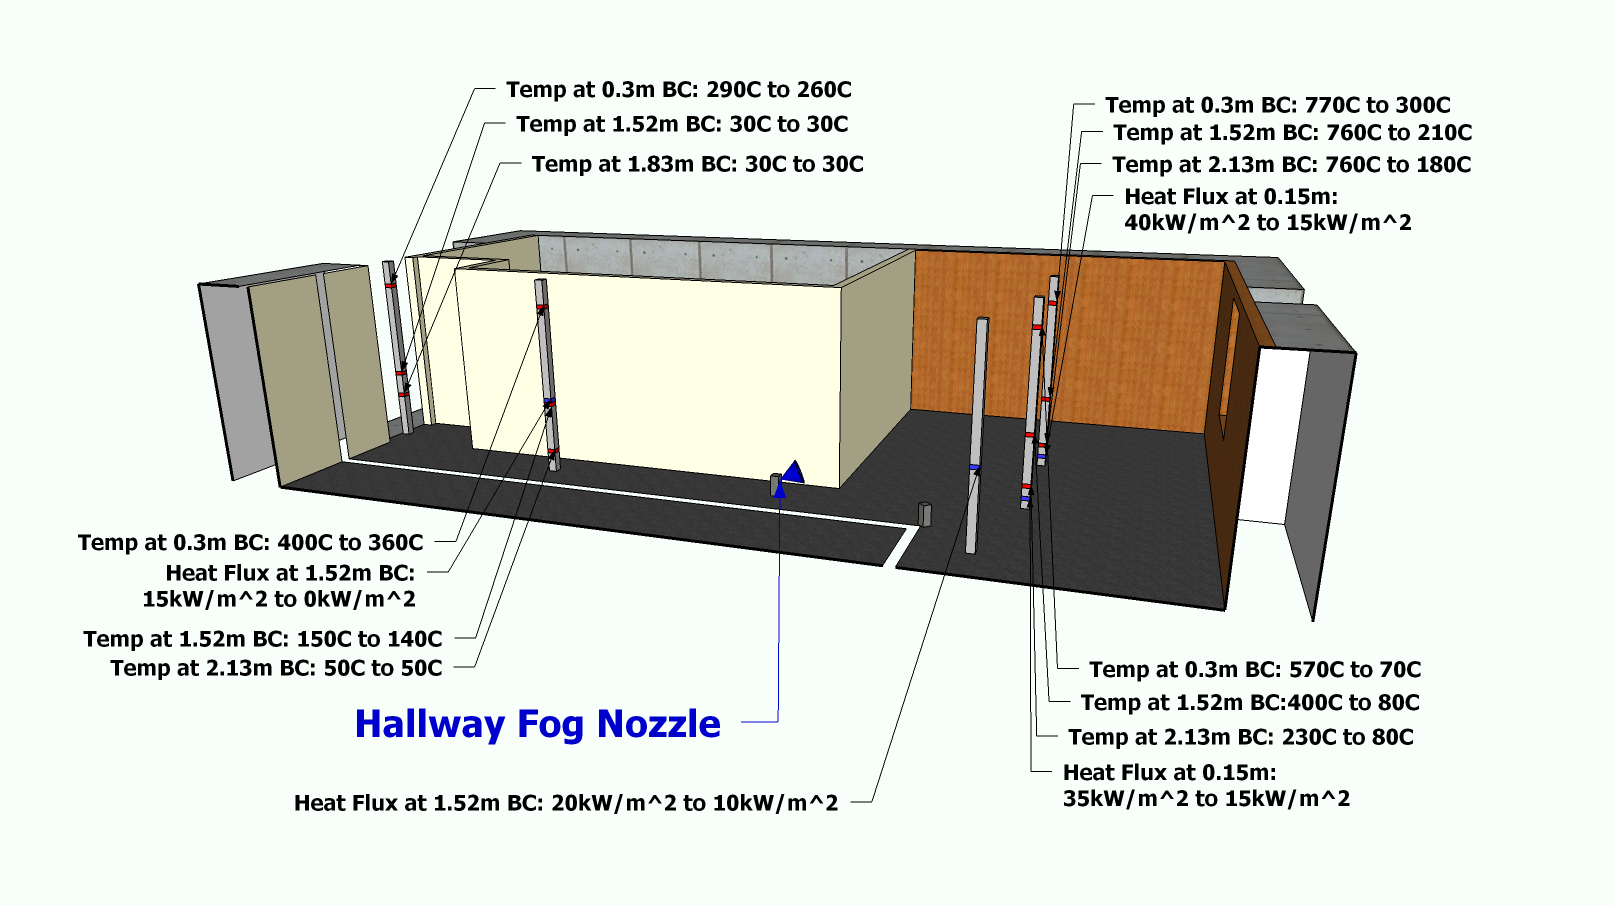
\includegraphics[width=6in]{../Figures/Pictures/Metric/DelCoFogTest2FirstSuppression}
	\caption{Test 2: Furniture Fuel Package, Water, 30$^{\circ}$ Fog, 120 gpm, First Suppression}
	\label{fig:Test_2_First_Suppression}
\end{figure}

\begin{figure}[!ht]
	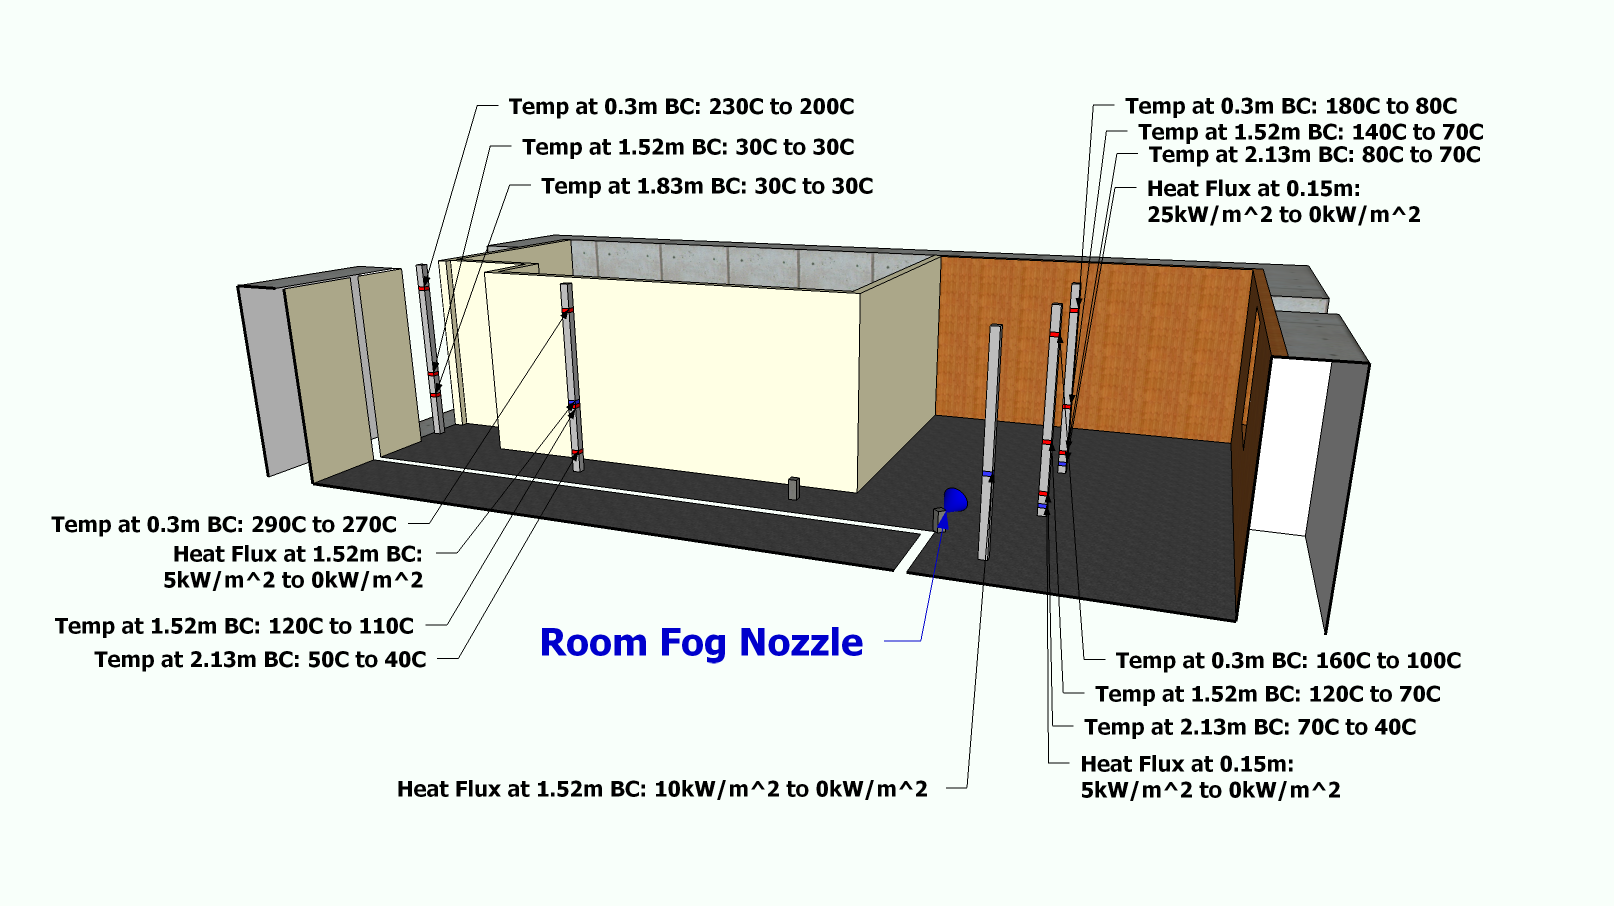
\includegraphics[width=6in]{../Figures/Pictures/Metric/DelCoFogTest2SecondSuppression}
	\caption{Test 2: Furniture Fuel Package, Water, 30$^{\circ}$ Fog, 120 gpm, Second Suppression}
	\label{fig:Test_2_Second_Suppression}
\end{figure}

\chapter{Discussion and Tactical Considerations}
\label{chap:Discussion_and_Tactical_Considerations}

\chapter{Summary}
\label{chap:Summary}


Smoke is Fuel. A ventilation limited (fuel rich) condition had developed prior to the failure of the window. Oxygen depleted combustion products, containing carbon dioxide, carbon monoxide and
unburned hydrocarbons filled the rooms of the structure. Once the window failed, the fresh air provided the oxygen needed to sustain the transition through flashover, which caused a significant increase in heat release rate.

Venting does not always equal cooling. In this experiment, post ventilation temperatures and heat fluxes all increased, due to the ventilation induced flashover. Fire induced flows. Velocities within the structure exceeded 5 m/s (11 mph), just due to the fire growth and the flow path that was set-up between the window opening and the corridor vent. Avoid the flow path. The directional nature of the fire gas flow was demonstrated with thermal conditions, both temperature and heat flux, which were twice as high in the ``flow'' portion of the
corridor as opposed to the ``static" portion of the corridor. Thermal conditions in the flow path were not consistent with firefighter survival.

The fuel load in the structure was the same for all of the experiments. Each of these experiments demonstrated a rapid transition to untenable conditions in the corridor, even for a firefighter in full PPE.

The externally applied water streams were implemented in three different ways; a fog stream across the face of the window opening, a fog stream into the window opening, and a solid water stream into the window opening.

These experiments demonstrated the ``extreme'' thermal conditions that can be generated by a ``simple room and contents'' fire and how these conditions can be extended along a flow path within a structure. The experiments also provided potential guidance for firefighters as a part of a fire size up and approach to the room of fire origin: note wind conditions in the area of the fire, look for ``pulsing flames'', examine smoke conditions around closed doors in the potential flow path, and maintain control of doors in the flow path.

Further research in actual buildings is required to fully understand the ability of firefighters to implement these tactics, to examine the thermal conditions throughout the structure such as in stairways, and to examine the interaction of these tactics with building ventilation strategies both natural and with positive pressure ventilation.


% \chapter{Appendix}
% \label{chap:Appendix}

% \section{Test 1 Figures}
% \label{subsec:Test_1_Figures}

% \subsection{Temperature}
% \label{subsec:Temperature}

% \begin{figure}[!ht]
% 	\includegraphics[width=6in]{../Figures/Temperature/FSE1_Eastside_Array}
% 	\caption{Test 1 (FSE1): Eastside Array}
% 	\label{fig:Test_1_Eastside_Array}
% \end{figure}

% \begin{figure}[!ht]
% 	\includegraphics[width=6in]{../Figures/Temperature/FSE1_Westside_Array}
% 	\caption{Test 1 (FSE1): Westside Array}
% 	\label{fig:Test_1_Westside_Array}
% \end{figure}

% \begin{figure}[!ht]
% 	\includegraphics[width=6in]{../Figures/Temperature/FSE1_Hallway_Array}
% 	\caption{Test 1 (FSE1): Hallway Array}
% 	\label{fig:Test_1_Hallway_Array}
% \end{figure}

% \begin{figure}[!ht]
% 	\includegraphics[width=6in]{../Figures/Temperature/FSE1_Doorway_Array}
% 	\caption{Test 1 (FSE1): Doorway Array}
% 	\label{fig:Test_1_Doorway_Array}
% \end{figure}

% \begin{figure}[!ht]
% 	\includegraphics[width=6in]{../Figures/Temperature/Suppression_FSE1_Eastside_Array}
% 	\caption{Test 1 (FSE1): Suppression Eastside Array}
% 	\label{fig:Test_1_Suppression_Eastside_Array}
% \end{figure}

% \begin{figure}[!ht]
% 	\includegraphics[width=6in]{../Figures/Temperature/Suppression_FSE1_Westside_Array}
% 	\caption{Test 1 (FSE1): Suppression Westside Array}
% 	\label{fig:Test_1_Suppression_Westside_Array}
% \end{figure}

% \begin{figure}[!ht]
% 	\includegraphics[width=6in]{../Figures/Temperature/Suppression_FSE1_Hallway_Array}
% 	\caption{Test 1 (FSE1): Suppression Hallway Array}
% 	\label{fig:Test_1_Suppression_Hallway_Array}
% \end{figure}

% \begin{figure}[!ht]
% 	\includegraphics[width=6in]{../Figures/Temperature/Suppression_FSE1_Doorway_Array}
% 	\caption{Test 1 (FSE1): Suppression Doorway Array}
% 	\label{fig:Test_1_Suppression_Doorway_Array}
% \end{figure}

% \subsection{Heat Flux}
% \label{subsec:Heat_Flux}

% \begin{figure}[!ht]
% 	\includegraphics[width=6in]{../Figures/Heat_Flux/FSE_Test_1_Heat_Flux_Eastside}
% 	\caption{Test 1 (FSE1): Eastside Heat Flux}
% 	\label{fig:Test_1_Eastside_Heat_Flux}
% \end{figure}

% \begin{figure}[!ht]
% 	\includegraphics[width=6in]{../Figures/Heat_Flux/FSE_Test_1_Heat_Flux_Westside}
% 	\caption{Test 1 (FSE1): Westside Heat Flux}
% 	\label{fig:Test_1_Westside_Heat_Flux}
% \end{figure}

% \begin{figure}[!ht]
% 	\includegraphics[width=6in]{../Figures/Heat_Flux/FSE_Test_1_Heat_Flux_Hallway}
% 	\caption{Test 1 (FSE1): Hallway Heat Flux}
% 	\label{fig:Test_1_Hallway_Heat_Flux}
% \end{figure}

% \begin{figure}[!ht]
% 	\includegraphics[width=6in]{../Figures/Heat_Flux/FSE_Test_1_Heat_Flux_Near_Fire_Room}
% 	\caption{Test 1 (FSE1): Heat Flux Near Fire Room}
% 	\label{fig:Test_1_Heat_Flux_Near_Fire_Room}
% \end{figure}

% \subsection{Velocity}
% \label{subsec:Velocity}

% \begin{figure}[!ht]
% 	\includegraphics[width=6in]{../Figures/Velocity/FSE_Test_1_Hallway_Velocity}
% 	\caption{Test 1 (FSE1): Hallway Velocity}
% 	\label{fig:Test_1_Hallway_Velocity}
% \end{figure}

% \begin{figure}[!ht]
% 	\includegraphics[width=6in]{../Figures/Velocity/FSE_Test_1_Doorway_Velocity}
% 	\caption{Test 1 (FSE1): Doorway Velocity}
% 	\label{fig:Test_1_Doorway_Velocity}
% \end{figure}

% \clearpage

% \section{Test 2 Figures}
% \label{subsec:Test_2_Figures}

% \subsection{Temperature}
% \label{subsec:Temperature}

% \begin{figure}[!ht]
% 	\includegraphics[width=6in]{../Figures/Temperature/FSW2_Eastside_Array}
% 	\caption{Test 2 (FSW2): Eastside Array}
% 	\label{fig:Test_2_Eastside_Array}
% \end{figure}

% \begin{figure}[!ht]
% 	\includegraphics[width=6in]{../Figures/Temperature/FSW2_Westside_Array}
% 	\caption{Test 2 (FSW2: Westside Array}
% 	\label{fig:Test_2_Westside_Array}
% \end{figure}

% \begin{figure}[!ht]
% 	\includegraphics[width=6in]{../Figures/Temperature/FSW2_Hallway_Array}
% 	\caption{Test 2 (FSW2): Hallway Array}
% 	\label{fig:Test_2_Hallway_Array}
% \end{figure}

% \begin{figure}[!ht]
% 	\includegraphics[width=6in]{../Figures/Temperature/FSW2_Doorway_Array}
% 	\caption{Test 2 (FSW2): Doorway Array}
% 	\label{fig:Test_2_Doorway_Array}
% \end{figure}

% \begin{figure}[!ht]
% 	\includegraphics[width=6in]{../Figures/Temperature/Suppression_FSW2_Eastside_Array}
% 	\caption{Test 2 (FSW2): Suppression Eastside Array}
% 	\label{fig:Test_2_Suppression_Eastside_Array}
% \end{figure}

% \begin{figure}[!ht]
% 	\includegraphics[width=6in]{../Figures/Temperature/Suppression_FSW2_Westside_Array}
% 	\caption{Test 2 (FSW2): Suppression Westside Array}
% 	\label{fig:Test_2_Suppression_Westside_Array}
% \end{figure}

% \begin{figure}[!ht]
% 	\includegraphics[width=6in]{../Figures/Temperature/Suppression_FSW2_Hallway_Array}
% 	\caption{Test 2 (FSW2): Suppression Hallway Array}
% 	\label{fig:Test_2_Suppression_Hallway_Array}
% \end{figure}

% \begin{figure}[!ht]
% 	\includegraphics[width=6in]{../Figures/Temperature/Suppression_FSW2_Doorway_Array}
% 	\caption{Test 2 (FSW2): Suppression Doorway Array}
% 	\label{fig:Test_2_Suppression_Doorway_Array}
% \end{figure}

% \subsection{Heat Flux}
% \label{subsec:Heat_Flux}

% \begin{figure}[!ht]
% 	\includegraphics[width=6in]{../Figures/Heat_Flux/FSW_Test_2_Heat_Flux_Eastside}
% 	\caption{Test 2 (FSW2): Eastside Heat Flux}
% 	\label{fig:Test_2_Eastside_Heat_Flux}
% \end{figure}

% \begin{figure}[!ht]
% 	\includegraphics[width=6in]{../Figures/Heat_Flux/FSW_Test_2_Heat_Flux_Westside}
% 	\caption{Test 2 (FSW2): Westside Heat Flux}
% 	\label{fig:Test_2_Westside_Heat_Flux}
% \end{figure}

% \begin{figure}[!ht]
% 	\includegraphics[width=6in]{../Figures/Heat_Flux/FSW_Test_2_Heat_Flux_Hallway}
% 	\caption{Test 2 (FSW2): Hallway Heat Flux}
% 	\label{fig:Test_2_Hallway_Heat_Flux}
% \end{figure}

% \begin{figure}[!ht]
% 	\includegraphics[width=6in]{../Figures/Heat_Flux/FSW_Test_2_Heat_Flux_Near_Fire_Room}
% 	\caption{Test 2 (FSW2): Heat Flux Near Fire Room}
% 	\label{fig:Test_2_Heat_Flux_Near_Fire_Room}
% \end{figure}

% \subsection{Velocity}
% \label{subsec:Velocity}

% \begin{figure}[!ht]
% 	\includegraphics[width=6in]{../Figures/Velocity/FSW_Test_2_Hallway_Velocity}
% 	\caption{Test 2 (FSW2): Hallway Velocity}
% 	\label{fig:Test_2_Hallway_Velocity}
% \end{figure}

% \begin{figure}[!ht]
% 	\includegraphics[width=6in]{../Figures/Velocity/FSW_Test_2_Doorway_Velocity}
% 	\caption{Test 2 (FSW2): Doorway Velocity}
% 	\label{fig:Test_2_Doorway_Velocity}
% \end{figure}

% \clearpage

% \section{Test 3 Figures}
% \label{subsec:Test_3_Figures}

% \subsection{Temperature}
% \label{subsec:Temperature}

% \begin{figure}[!ht]
% 	\includegraphics[width=6in]{../Figures/Temperature/FSW3_Eastside_Array}
% 	\caption{Test 3 (FSW3): Eastside Array}
% 	\label{fig:Test_3_Eastside_Array}
% \end{figure}

% \begin{figure}[!ht]
% 	\includegraphics[width=6in]{../Figures/Temperature/FSW3_Westside_Array}
% 	\caption{Test 3 (FSW3: Westside Array}
% 	\label{fig:Test_3_Westside_Array}
% \end{figure}

% \begin{figure}[!ht]
% 	\includegraphics[width=6in]{../Figures/Temperature/FSW3_Hallway_Array}
% 	\caption{Test 3 (FSW3): Hallway Array}
% 	\label{fig:Test_3_Hallway_Array}
% \end{figure}

% \begin{figure}[!ht]
% 	\includegraphics[width=6in]{../Figures/Temperature/FSW3_Doorway_Array}
% 	\caption{Test 3 (FSW3): Doorway Array}
% 	\label{fig:Test_3_Doorway_Array}
% \end{figure}

% \begin{figure}[!ht]
% 	\includegraphics[width=6in]{../Figures/Temperature/Suppression_FSW3_Eastside_Array}
% 	\caption{Test 3 (FSW3): Suppression Eastside Array}
% 	\label{fig:Test_3_Suppression_Eastside_Array}
% \end{figure}

% \begin{figure}[!ht]
% 	\includegraphics[width=6in]{../Figures/Temperature/Suppression_FSW3_Westside_Array}
% 	\caption{Test 3 (FSW3): Suppression Westside Array}
% 	\label{fig:Test_3_Suppression_Westside_Array}
% \end{figure}

% \begin{figure}[!ht]
% 	\includegraphics[width=6in]{../Figures/Temperature/Suppression_FSW3_Hallway_Array}
% 	\caption{Test 3 (FSW3): Suppression Hallway Array}
% 	\label{fig:Test_3_Suppression_Hallway_Array}
% \end{figure}

% \begin{figure}[!ht]
% 	\includegraphics[width=6in]{../Figures/Temperature/Suppression_FSW3_Doorway_Array}
% 	\caption{Test 3 (FSW3): Suppression Doorway Array}
% 	\label{fig:Test_3_Suppression_Doorway_Array}
% \end{figure}

% \subsection{Heat Flux}
% \label{subsec:Heat_Flux}

% \begin{figure}[!ht]
% 	\includegraphics[width=6in]{../Figures/Heat_Flux/FSW_Test_3_Heat_Flux_Eastside}
% 	\caption{Test 3 (FSW3): Eastside Heat Flux}
% 	\label{fig:Test_3_Eastside_Heat_Flux}
% \end{figure}

% \begin{figure}[!ht]
% 	\includegraphics[width=6in]{../Figures/Heat_Flux/FSW_Test_3_Heat_Flux_Westside}
% 	\caption{Test 3 (FSW3): Westside Heat Flux}
% 	\label{fig:Test_3_Westside_Heat_Flux}
% \end{figure}

% \begin{figure}[!ht]
% 	\includegraphics[width=6in]{../Figures/Heat_Flux/FSW_Test_3_Heat_Flux_Hallway}
% 	\caption{Test 3 (FSW3): Hallway Heat Flux}
% 	\label{fig:Test_3_Hallway_Heat_Flux}
% \end{figure}

% \begin{figure}[!ht]
% 	\includegraphics[width=6in]{../Figures/Heat_Flux/FSW_Test_3_Heat_Flux_Near_Fire_Room}
% 	\caption{Test 3 (FSW3): Heat Flux Near Fire Room}
% 	\label{fig:Test_3_Heat_Flux_Near_Fire_Room}
% \end{figure}

% \subsection{Velocity}
% \label{subsec:Velocity}

% \begin{figure}[!ht]
% 	\includegraphics[width=6in]{../Figures/Velocity/FSW_Test_3_Hallway_Velocity}
% 	\caption{Test 3 (FSW3): Hallway Velocity}
% 	\label{fig:Test_3_Hallway_Velocity}
% \end{figure}

% \begin{figure}[!ht]
% 	\includegraphics[width=6in]{../Figures/Velocity/FSW_Test_3_Doorway_Velocity}
% 	\caption{Test 3 (FSW3): Doorway Velocity}
% 	\label{fig:Test_3_Doorway_Velocity}
% \end{figure}

% \clearpage

% \section{Test 4 Figures}
% \label{subsec:Test_4_Figures}

% \subsection{Temperature}
% \label{subsec:Temperature}

% \begin{figure}[!ht]
% 	\includegraphics[width=6in]{../Figures/Temperature/FSE4_Eastside_Array}
% 	\caption{Test 4 (FSE4): Eastside Array}
% 	\label{fig:Test_4_Eastside_Array}
% \end{figure}

% \begin{figure}[!ht]
% 	\includegraphics[width=6in]{../Figures/Temperature/FSE4_Westside_Array}
% 	\caption{Test 4 (FSE4): Westside Array}
% 	\label{fig:Test_4_Westside_Array}
% \end{figure}

% \begin{figure}[!ht]
% 	\includegraphics[width=6in]{../Figures/Temperature/FSE4_Hallway_Array}
% 	\caption{Test 4 (FSE4): Hallway Array}
% 	\label{fig:Test_4_Hallway_Array}
% \end{figure}

% \begin{figure}[!ht]
% 	\includegraphics[width=6in]{../Figures/Temperature/FSE4_Doorway_Array}
% 	\caption{Test 4 (FSE4): Doorway Array}
% 	\label{fig:Test_4_Doorway_Array}
% \end{figure}

% \begin{figure}[!ht]
% 	\includegraphics[width=6in]{../Figures/Temperature/Suppression_FSE4_Eastside_Array}
% 	\caption{Test 4 (FSE4): Suppression Eastside Array}
% 	\label{fig:Test_4_Suppression_Eastside_Array}
% \end{figure}

% \begin{figure}[!ht]
% 	\includegraphics[width=6in]{../Figures/Temperature/Suppression_FSE4_Westside_Array}
% 	\caption{Test 4 (FSE4): Suppression Westside Array}
% 	\label{fig:Test_4_Suppression_Westside_Array}
% \end{figure}

% \begin{figure}[!ht]
% 	\includegraphics[width=6in]{../Figures/Temperature/Suppression_FSE4_Hallway_Array}
% 	\caption{Test 4 (FSE4): Suppression Hallway Array}
% 	\label{fig:Test_4_Suppression_Hallway_Array}
% \end{figure}

% \begin{figure}[!ht]
% 	\includegraphics[width=6in]{../Figures/Temperature/Suppression_FSE4_Doorway_Array}
% 	\caption{Test 4 (FSE4): Suppression Doorway Array}
% 	\label{fig:Test_4_Suppression_Doorway_Array}
% \end{figure}

% \subsection{Heat Flux}
% \label{subsec:Heat_Flux}

% \begin{figure}[!ht]
% 	\includegraphics[width=6in]{../Figures/Heat_Flux/FSE_Test_4_Heat_Flux_Eastside}
% 	\caption{Test 4 (FSE4): Eastside Heat Flux}
% 	\label{fig:Test_4_Eastside_Heat_Flux}
% \end{figure}

% \begin{figure}[!ht]
% 	\includegraphics[width=6in]{../Figures/Heat_Flux/FSE_Test_4_Heat_Flux_Westside}
% 	\caption{Test 4 (FSE4): Westside Heat Flux}
% 	\label{fig:Test_4_Westside_Heat_Flux}
% \end{figure}

% \begin{figure}[!ht]
% 	\includegraphics[width=6in]{../Figures/Heat_Flux/FSE_Test_4_Heat_Flux_Hallway}
% 	\caption{Test 4 (FSE4): Hallway Heat Flux}
% 	\label{fig:Test_4_Hallway_Heat_Flux}
% \end{figure}

% \begin{figure}[!ht]
% 	\includegraphics[width=6in]{../Figures/Heat_Flux/FSE_Test_4_Heat_Flux_Near_Fire_Room}
% 	\caption{Test 4 (FSE4): Heat Flux Near Fire Room}
% 	\label{fig:Test_4_Heat_Flux_Near_Fire_Room}
% \end{figure}

% \subsection{Velocity}
% \label{subsec:Velocity}

% \begin{figure}[!ht]
% 	\includegraphics[width=6in]{../Figures/Velocity/FSE_Test_4_Hallway_Velocity}
% 	\caption{Test 4 (FSE4): Hallway Velocity}
% 	\label{fig:Test_4_Hallway_Velocity}
% \end{figure}

% \begin{figure}[!ht]
% 	\includegraphics[width=6in]{../Figures/Velocity/FSE_Test_4_Doorway_Velocity}
% 	\caption{Test 4 (FSE4): Doorway Velocity}
% 	\label{fig:Test_4_Doorway_Velocity}
% \end{figure}

% \clearpage

% \section{Test 5 Figures}
% \label{subsec:Test_5_Figures}

% \subsection{Temperature}
% \label{subsec:Temperature}

% \begin{figure}[!ht]
% 	\includegraphics[width=6in]{../Figures/Temperature/FSE5_Eastside_Array}
% 	\caption{Test 5 (FSE5): Eastside Array}
% 	\label{fig:Test_5_Eastside_Array}
% \end{figure}

% \begin{figure}[!ht]
% 	\includegraphics[width=6in]{../Figures/Temperature/FSE5_Westside_Array}
% 	\caption{Test 5 (FSE5): Westside Array}
% 	\label{fig:Test_5_Westside_Array}
% \end{figure}

% \begin{figure}[!ht]
% 	\includegraphics[width=6in]{../Figures/Temperature/FSE5_Hallway_Array}
% 	\caption{Test 5 (FSE5): Hallway Array}
% 	\label{fig:Test_5_Hallway_Array}
% \end{figure}

% \begin{figure}[!ht]
% 	\includegraphics[width=6in]{../Figures/Temperature/FSE5_Doorway_Array}
% 	\caption{Test 5 (FSE5): Doorway Array}
% 	\label{fig:Test_5_Doorway_Array}
% \end{figure}

% \begin{figure}[!ht]
% 	\includegraphics[width=6in]{../Figures/Temperature/Suppression_FSE5_Eastside_Array}
% 	\caption{Test 5 (FSE5): Suppression Eastside Array}
% 	\label{fig:Test_5_Suppression_Eastside_Array}
% \end{figure}

% \begin{figure}[!ht]
% 	\includegraphics[width=6in]{../Figures/Temperature/Suppression_FSE5_Westside_Array}
% 	\caption{Test 5 (FSE5): Suppression Westside Array}
% 	\label{fig:Test_5_Suppression_Westside_Array}
% \end{figure}

% \begin{figure}[!ht]
% 	\includegraphics[width=6in]{../Figures/Temperature/Suppression_FSE5_Hallway_Array}
% 	\caption{Test 5 (FSE5): Suppression Hallway Array}
% 	\label{fig:Test_5_Suppression_Hallway_Array}
% \end{figure}

% \begin{figure}[!ht]
% 	\includegraphics[width=6in]{../Figures/Temperature/Suppression_FSE5_Doorway_Array}
% 	\caption{Test 5 (FSE5): Suppression Doorway Array}
% 	\label{fig:Test_5_Suppression_Doorway_Array}
% \end{figure}

% \subsection{Heat Flux}
% \label{subsec:Heat_Flux}

% \begin{figure}[!ht]
% 	\includegraphics[width=6in]{../Figures/Heat_Flux/FSE_Test_5_Heat_Flux_Eastside}
% 	\caption{Test 5 (FSE5): Eastside Heat Flux}
% 	\label{fig:Test_5_Eastside_Heat_Flux}
% \end{figure}

% \begin{figure}[!ht]
% 	\includegraphics[width=6in]{../Figures/Heat_Flux/FSE_Test_5_Heat_Flux_Westside}
% 	\caption{Test 5 (FSE5): Westside Heat Flux}
% 	\label{fig:Test_5_Westside_Heat_Flux}
% \end{figure}

% \begin{figure}[!ht]
% 	\includegraphics[width=6in]{../Figures/Heat_Flux/FSE_Test_5_Heat_Flux_Hallway}
% 	\caption{Test 5 (FSE5): Hallway Heat Flux}
% 	\label{fig:Test_5_Hallway_Heat_Flux}
% \end{figure}

% \begin{figure}[!ht]
% 	\includegraphics[width=6in]{../Figures/Heat_Flux/FSE_Test_5_Heat_Flux_Near_Fire_Room}
% 	\caption{Test 5 (FSE5): Heat Flux Near Fire Room}
% 	\label{fig:Test_5_Heat_Flux_Near_Fire_Room}
% \end{figure}

% \subsection{Velocity}
% \label{subsec:Velocity}

% \begin{figure}[!ht]
% 	\includegraphics[width=6in]{../Figures/Velocity/FSE_Test_5_Hallway_Velocity}
% 	\caption{Test 5 (FSE5): Hallway Velocity}
% 	\label{fig:Test_5_Hallway_Velocity}
% \end{figure}

% \begin{figure}[!ht]
% 	\includegraphics[width=6in]{../Figures/Velocity/FSE_Test_5_Doorway_Velocity}
% 	\caption{Test 5 (FSE5): Doorway Velocity}
% 	\label{fig:Test_5_Doorway_Velocity}
% \end{figure}

% \clearpage

% \section{Test 6 Figures}
% \label{subsec:Test_6_Figures}

% \subsection{Temperature}
% \label{subsec:Temperature}

% \begin{figure}[!ht]
% 	\includegraphics[width=6in]{../Figures/Temperature/FSW6_Eastside_Array}
% 	\caption{Test 6 (FSW6): Eastside Array}
% 	\label{fig:Test_6_Eastside_Array}
% \end{figure}

% \begin{figure}[!ht]
% 	\includegraphics[width=6in]{../Figures/Temperature/FSW6_Westside_Array}
% 	\caption{Test 6 (FSW6: Westside Array}
% 	\label{fig:Test_6_Westside_Array}
% \end{figure}

% \begin{figure}[!ht]
% 	\includegraphics[width=6in]{../Figures/Temperature/FSW6_Hallway_Array}
% 	\caption{Test 6 (FSW6): Hallway Array}
% 	\label{fig:Test_6_Hallway_Array}
% \end{figure}

% \begin{figure}[!ht]
% 	\includegraphics[width=6in]{../Figures/Temperature/FSW6_Doorway_Array}
% 	\caption{Test 6 (FSW6): Doorway Array}
% 	\label{fig:Test_6_Doorway_Array}
% \end{figure}

% \begin{figure}[!ht]
% 	\includegraphics[width=6in]{../Figures/Temperature/Suppression_FSW6_Eastside_Array}
% 	\caption{Test 6 (FSW6): Suppression Eastside Array}
% 	\label{fig:Test_6_Suppression_Eastside_Array}
% \end{figure}

% \begin{figure}[!ht]
% 	\includegraphics[width=6in]{../Figures/Temperature/Suppression_FSW6_Westside_Array}
% 	\caption{Test 6 (FSW6): Suppression Westside Array}
% 	\label{fig:Test_6_Suppression_Westside_Array}
% \end{figure}

% \begin{figure}[!ht]
% 	\includegraphics[width=6in]{../Figures/Temperature/Suppression_FSW6_Hallway_Array}
% 	\caption{Test 6 (FSW6): Suppression Hallway Array}
% 	\label{fig:Test_6_Suppression_Hallway_Array}
% \end{figure}

% \begin{figure}[!ht]
% 	\includegraphics[width=6in]{../Figures/Temperature/Suppression_FSW6_Doorway_Array}
% 	\caption{Test 6 (FSW6): Suppression Doorway Array}
% 	\label{fig:Test_6_Suppression_Doorway_Array}
% \end{figure}

% \subsection{Heat Flux}
% \label{subsec:Heat_Flux}

% \begin{figure}[!ht]
% 	\includegraphics[width=6in]{../Figures/Heat_Flux/FSW_Test_6_Heat_Flux_Eastside}
% 	\caption{Test 6 (FSW6): Eastside Heat Flux}
% 	\label{fig:Test_6_Eastside_Heat_Flux}
% \end{figure}

% \begin{figure}[!ht]
% 	\includegraphics[width=6in]{../Figures/Heat_Flux/FSW_Test_6_Heat_Flux_Westside}
% 	\caption{Test 6 (FSW6): Westside Heat Flux}
% 	\label{fig:Test_6_Westside_Heat_Flux}
% \end{figure}

% \begin{figure}[!ht]
% 	\includegraphics[width=6in]{../Figures/Heat_Flux/FSW_Test_6_Heat_Flux_Hallway}
% 	\caption{Test 6 (FSW6): Hallway Heat Flux}
% 	\label{fig:Test_6_Hallway_Heat_Flux}
% \end{figure}

% \begin{figure}[!ht]
% 	\includegraphics[width=6in]{../Figures/Heat_Flux/FSW_Test_6_Heat_Flux_Near_Fire_Room}
% 	\caption{Test 6 (FSW6): Heat Flux Near Fire Room}
% 	\label{fig:Test_6_Heat_Flux_Near_Fire_Room}
% \end{figure}

% \subsection{Velocity}
% \label{subsec:Velocity}

% \begin{figure}[!ht]
% 	\includegraphics[width=6in]{../Figures/Velocity/FSW_Test_6_Hallway_Velocity}
% 	\caption{Test 6 (FSW6): Hallway Velocity}
% 	\label{fig:Test_6_Hallway_Velocity}
% \end{figure}

% \begin{figure}[!ht]
% 	\includegraphics[width=6in]{../Figures/Velocity/FSW_Test_6_Doorway_Velocity}
% 	\caption{Test 6 (FSW6): Doorway Velocity}
% 	\label{fig:Test_6_Doorway_Velocity}
% \end{figure}

% \clearpage

% \section{Test 7 Figures}
% \label{subsec:Test_7_Figures}

% \subsection{Temperature}
% \label{subsec:Temperature}

% \begin{figure}[!ht]
% 	\includegraphics[width=6in]{../Figures/Temperature/FSW7_Eastside_Array}
% 	\caption{Test 7 (FSW7): Eastside Array}
% 	\label{fig:Test_7_Eastside_Array}
% \end{figure}

% \begin{figure}[!ht]
% 	\includegraphics[width=6in]{../Figures/Temperature/FSW7_Westside_Array}
% 	\caption{Test 7 (FSW7: Westside Array}
% 	\label{fig:Test_7_Westside_Array}
% \end{figure}

% \begin{figure}[!ht]
% 	\includegraphics[width=6in]{../Figures/Temperature/FSW7_Hallway_Array}
% 	\caption{Test 7 (FSW7): Hallway Array}
% 	\label{fig:Test_7_Hallway_Array}
% \end{figure}

% \begin{figure}[!ht]
% 	\includegraphics[width=6in]{../Figures/Temperature/FSW7_Doorway_Array}
% 	\caption{Test 7 (FSW7): Doorway Array}
% 	\label{fig:Test_7_Doorway_Array}
% \end{figure}

% \begin{figure}[!ht]
% 	\includegraphics[width=6in]{../Figures/Temperature/Suppression_FSW7_Eastside_Array}
% 	\caption{Test 7 (FSW7): Suppression Eastside Array}
% 	\label{fig:Test_7_Suppression_Eastside_Array}
% \end{figure}

% \begin{figure}[!ht]
% 	\includegraphics[width=6in]{../Figures/Temperature/Suppression_FSW7_Westside_Array}
% 	\caption{Test 7 (FSW7): Suppression Westside Array}
% 	\label{fig:Test_7_Suppression_Westside_Array}
% \end{figure}

% \begin{figure}[!ht]
% 	\includegraphics[width=6in]{../Figures/Temperature/Suppression_FSW7_Hallway_Array}
% 	\caption{Test 7 (FSW7): Suppression Hallway Array}
% 	\label{fig:Test_7_Suppression_Hallway_Array}
% \end{figure}

% \begin{figure}[!ht]
% 	\includegraphics[width=6in]{../Figures/Temperature/Suppression_FSW7_Doorway_Array}
% 	\caption{Test 7 (FSW7): Suppression Doorway Array}
% 	\label{fig:Test_7_Suppression_Doorway_Array}
% \end{figure}

% \subsection{Heat Flux}
% \label{subsec:Heat_Flux}

% \begin{figure}[!ht]
% 	\includegraphics[width=6in]{../Figures/Heat_Flux/FSW_Test_7_Heat_Flux_Eastside}
% 	\caption{Test 7 (FSW7): Eastside Heat Flux}
% 	\label{fig:Test_7_Eastside_Heat_Flux}
% \end{figure}

% \begin{figure}[!ht]
% 	\includegraphics[width=6in]{../Figures/Heat_Flux/FSW_Test_7_Heat_Flux_Westside}
% 	\caption{Test 7 (FSW7): Westside Heat Flux}
% 	\label{fig:Test_7_Westside_Heat_Flux}
% \end{figure}

% \begin{figure}[!ht]
% 	\includegraphics[width=6in]{../Figures/Heat_Flux/FSW_Test_7_Heat_Flux_Hallway}
% 	\caption{Test 7 (FSW7): Hallway Heat Flux}
% 	\label{fig:Test_7_Hallway_Heat_Flux}
% \end{figure}

% \begin{figure}[!ht]
% 	\includegraphics[width=6in]{../Figures/Heat_Flux/FSW_Test_7_Heat_Flux_Near_Fire_Room}
% 	\caption{Test 7 (FSW7): Heat Flux Near Fire Room}
% 	\label{fig:Test_7_Heat_Flux_Near_Fire_Room}
% \end{figure}

% \subsection{Velocity}
% \label{subsec:Velocity}

% \begin{figure}[!ht]
% 	\includegraphics[width=6in]{../Figures/Velocity/FSW_Test_7_Hallway_Velocity}
% 	\caption{Test 7 (FSW7): Hallway Velocity}
% 	\label{fig:Test_7_Hallway_Velocity}
% \end{figure}

% \begin{figure}[!ht]
% 	\includegraphics[width=6in]{../Figures/Velocity/FSW_Test_7_Doorway_Velocity}
% 	\caption{Test 7 (FSW7): Doorway Velocity}
% 	\label{fig:Test_7_Doorway_Velocity}
% \end{figure}

% \clearpage

% \section{Test 8 Figures}
% \label{subsec:Test_8_Figures}

% \subsection{Temperature}
% \label{subsec:Temperature}

% \begin{figure}[!ht]
% 	\includegraphics[width=6in]{../Figures/Temperature/FSE8_Eastside_Array}
% 	\caption{Test 8 (FSE8): Eastside Array}
% 	\label{fig:Test_8_Eastside_Array}
% \end{figure}

% \begin{figure}[!ht]
% 	\includegraphics[width=6in]{../Figures/Temperature/FSE8_Westside_Array}
% 	\caption{Test 8 (FSE8): Westside Array}
% 	\label{fig:Test_8_Westside_Array}
% \end{figure}

% \begin{figure}[!ht]
% 	\includegraphics[width=6in]{../Figures/Temperature/FSE8_Hallway_Array}
% 	\caption{Test 8 (FSE8): Hallway Array}
% 	\label{fig:Test_8_Hallway_Array}
% \end{figure}

% \begin{figure}[!ht]
% 	\includegraphics[width=6in]{../Figures/Temperature/FSE8_Doorway_Array}
% 	\caption{Test 8 (FSE8): Doorway Array}
% 	\label{fig:Test_8_Doorway_Array}
% \end{figure}

% \begin{figure}[!ht]
% 	\includegraphics[width=6in]{../Figures/Temperature/Suppression_FSE8_Eastside_Array}
% 	\caption{Test 8 (FSE8): Suppression Eastside Array}
% 	\label{fig:Test_8_Suppression_Eastside_Array}
% \end{figure}

% \begin{figure}[!ht]
% 	\includegraphics[width=6in]{../Figures/Temperature/Suppression_FSE8_Westside_Array}
% 	\caption{Test 8 (FSE8): Suppression Westside Array}
% 	\label{fig:Test_8_Suppression_Westside_Array}
% \end{figure}

% \begin{figure}[!ht]
% 	\includegraphics[width=6in]{../Figures/Temperature/Suppression_FSE8_Hallway_Array}
% 	\caption{Test 8 (FSE8): Suppression Hallway Array}
% 	\label{fig:Test_8_Suppression_Hallway_Array}
% \end{figure}

% \begin{figure}[!ht]
% 	\includegraphics[width=6in]{../Figures/Temperature/Suppression_FSE8_Doorway_Array}
% 	\caption{Test 8 (FSE8): Suppression Doorway Array}
% 	\label{fig:Test_8_Suppression_Doorway_Array}
% \end{figure}

% \subsection{Heat Flux}
% \label{subsec:Heat_Flux}

% \begin{figure}[!ht]
% 	\includegraphics[width=6in]{../Figures/Heat_Flux/FSE_Test_8_Heat_Flux_Eastside}
% 	\caption{Test 8 (FSE8): Eastside Heat Flux}
% 	\label{fig:Test_8_Eastside_Heat_Flux}
% \end{figure}

% \begin{figure}[!ht]
% 	\includegraphics[width=6in]{../Figures/Heat_Flux/FSE_Test_8_Heat_Flux_Westside}
% 	\caption{Test 8 (FSE8): Westside Heat Flux}
% 	\label{fig:Test_8_Westside_Heat_Flux}
% \end{figure}

% \begin{figure}[!ht]
% 	\includegraphics[width=6in]{../Figures/Heat_Flux/FSE_Test_8_Heat_Flux_Hallway}
% 	\caption{Test 8 (FSE8): Hallway Heat Flux}
% 	\label{fig:Test_8_Hallway_Heat_Flux}
% \end{figure}

% \begin{figure}[!ht]
% 	\includegraphics[width=6in]{../Figures/Heat_Flux/FSE_Test_8_Heat_Flux_Near_Fire_Room}
% 	\caption{Test 8 (FSE8): Heat Flux Near Fire Room}
% 	\label{fig:Test_8_Heat_Flux_Near_Fire_Room}
% \end{figure}

% \subsection{Velocity}
% \label{subsec:Velocity}

% \begin{figure}[!ht]
% 	\includegraphics[width=6in]{../Figures/Velocity/FSE_Test_8_Hallway_Velocity}
% 	\caption{Test 8 (FSE8): Hallway Velocity}
% 	\label{fig:Test_8_Hallway_Velocity}
% \end{figure}

% \begin{figure}[!ht]
% 	\includegraphics[width=6in]{../Figures/Velocity/FSE_Test_8_Doorway_Velocity}
% 	\caption{Test 8 (FSE8): Doorway Velocity}
% 	\label{fig:Test_8_Doorway_Velocity}
% \end{figure}

\clearpage

\bibliography{../../../Bibliography/FDS_refs,../../../Bibliography/FDS_general}

\appendix

\chapter{Fuel Load Details}
\label{app:fuel_loads}


\chapter{Spray Density Figures}
\label{app:spray_density}

\begin{figure}[!ht]
	\includegraphics[width=4in]{../Figures/Bars/BB2}
	\caption{Burn Building Test 2}
	\label{fig:Burn_Building_Test_2}
\end{figure}

\begin{figure}[!ht]
	\includegraphics[width=4in]{../Figures/Bars/BB3}
	\caption{Burn Building Test 3}
	\label{fig:Burn_Building_Test_3}
\end{figure}

\begin{figure}[!ht]
	\includegraphics[width=4in]{../Figures/Bars/BB4}
	\caption{Burn Building Test 4}
	\label{fig:Burn_Building_Test_4}
\end{figure}

\begin{figure}[!ht]
	\includegraphics[width=4in]{../Figures/Bars/BB5}
	\caption{Burn Building Test 5}
	\label{fig:Burn_Building_Test_5}
\end{figure}

\clearpage

\begin{figure}[!ht]
	\includegraphics[width=4in]{../Figures/Bars/BB6}
	\caption{Burn Building Test 6}
	\label{fig:Burn_Building_Test_6}
\end{figure}

\begin{figure}[!ht]
	\includegraphics[width=4in]{../Figures/Bars/BB8}
	\caption{Burn Building Test 8}
	\label{fig:Burn_Building_Test_8}
\end{figure}

\begin{figure}[!ht]
	\includegraphics[width=4in]{../Figures/Bars/BB9}
	\caption{Burn Building Test 9}
	\label{fig:Burn_Building_Test_9}
\end{figure}

\begin{figure}[!ht]
	\includegraphics[width=4in]{../Figures/Bars/BB10}
	\caption{Burn Building Test 10}
	\label{fig:Burn_Building_Test_10}
\end{figure}

\clearpage

\begin{figure}[!ht]
	\includegraphics[width=4in]{../Figures/Bars/BB11}
	\caption{Burn Building Test 11}
	\label{fig:Burn_Building_Test_11}
\end{figure}

\begin{figure}[!ht]
	\includegraphics[width=4in]{../Figures/Bars/BB12}
	\caption{Burn Building Test 12}
	\label{fig:Burn_Building_Test_12}
\end{figure}

\begin{figure}[!ht]
	\includegraphics[width=4in]{../Figures/Bars/BB13}
	\caption{Burn Building Test 13}
	\label{fig:Burn_Building_Test_13}
\end{figure}

\begin{figure}[!ht]
	\includegraphics[width=4in]{../Figures/Bars/BB14}
	\caption{Burn Building Test 14}
	\label{fig:Burn_Building_Test_14}
\end{figure}

\clearpage

\begin{figure}[!ht]
	\includegraphics[width=4in]{../Figures/Bars/BB15}
	\caption{Burn Building Test 15}
	\label{fig:Burn_Building_Test_15}
\end{figure}

\begin{figure}[!ht]
	\includegraphics[width=4in]{../Figures/Bars/BB16}
	\caption{Burn Building Test 16}
	\label{fig:Burn_Building_Test_16}
\end{figure}

\begin{figure}[!ht]
	\includegraphics[width=4in]{../Figures/Bars/BB17}
	\caption{Burn Building Test 17}
	\label{fig:Burn_Building_Test_17}
\end{figure}

\begin{figure}[!ht]
	\includegraphics[width=4in]{../Figures/Bars/BB18}
	\caption{Burn Building Test 18}
	\label{fig:Burn_Building_Test_18}
\end{figure}

\clearpage

\begin{figure}[!ht]
	\includegraphics[width=4in]{../Figures/Bars/BB19}
	\caption{Burn Building Test 19}
	\label{fig:Burn_Building_Test_19}
\end{figure}

\begin{figure}[!ht]
	\includegraphics[width=4in]{../Figures/Bars/BB20}
	\caption{Burn Building Test 20}
	\label{fig:Burn_Building_Test_20}
\end{figure}

\begin{figure}[!ht]
	\includegraphics[width=4in]{../Figures/Bars/BB21}
	\caption{Burn Building Test 21}
	\label{fig:Burn_Building_Test_21}
\end{figure}

\begin{figure}[!ht]
	\includegraphics[width=4in]{../Figures/Bars/ES_1}
	\caption{Experimental Structures Test 1}
	\label{fig:Experimental_Structures_Test_1}
\end{figure}

\clearpage

\begin{figure}[!ht]
	\includegraphics[width=4in]{../Figures/Bars/ES_2}
	\caption{Experimental Structures Test 2}
	\label{fig:Experimental_Structures_Test_2}
\end{figure}

\begin{figure}[!ht]
	\includegraphics[width=4in]{../Figures/Bars/ES_3}
	\caption{Experimental Structures Test 3}
	\label{fig:Experimental_Structures_Test_3}
\end{figure}

\begin{figure}[!ht]
	\includegraphics[width=4in]{../Figures/Bars/ES_4}
	\caption{Experimental Structures Test 4}
	\label{fig:Experimental_Structures_Test_4}
\end{figure}

\begin{figure}[!ht]
	\includegraphics[width=4in]{../Figures/Bars/ES_5}
	\caption{Experimental Structures Test 5}
	\label{fig:Experimental_Structures_Test_5}
\end{figure}

\clearpage

\begin{figure}[!ht]
	\includegraphics[width=4in]{../Figures/Bars/ES_6}
	\caption{Experimental Structures Test 6}
	\label{fig:Experimental_Structures_Test_6}
\end{figure}

\begin{figure}[!ht]
	\includegraphics[width=4in]{../Figures/Bars/ES_7}
	\caption{Experimental Structures Test 7}
	\label{fig:Experimental_Structures_Test_7}
\end{figure}

\begin{figure}[!ht]
	\includegraphics[width=4in]{../Figures/Bars/ES_72}
	\caption{Experimental Structures Test 7.2}
	\label{fig:Experimental_Structures_Test_7.2}
\end{figure}

\begin{figure}[!ht]
	\includegraphics[width=4in]{../Figures/Bars/ES_8}
	\caption{Experimental Structures Test 8}
	\label{fig:Experimental_Structures_Test_8}
\end{figure}

\clearpage

\begin{figure}[!ht]
	\includegraphics[width=4in]{../Figures/Bars/ES_9}
	\caption{Experimental Structures Test 9}
	\label{fig:Experimental_Structures_Test_9}
\end{figure}

\begin{figure}[!ht]
	\includegraphics[width=4in]{../Figures/Bars/ES_10}
	\caption{Experimental Structures Test 10}
	\label{fig:Experimental_Structures_Test_10}
\end{figure}

\begin{figure}[!ht]
	\includegraphics[width=4in]{../Figures/Bars/ES_11}
	\caption{Experimental Structures Test 11}
	\label{fig:Experimental_Structures_Test_11}
\end{figure}


\chapter{Fire Suppression Figures}
\label{app:fire_suppression}

\section{Furniture Fuel Package}
\label{appsubsec:Furniture_Fuel_Package}

\begin{figure}[!ht]
	\includegraphics[width=6in]{../Figures/Pictures/Metric/DelCoSSTest3FirstSuppression}
	\caption{Test 3: Furniture Fuel Package, CAFS, 7/8" Smooth Bore, 120 gpm/60 cfm, First Suppression}
	\label{fig:Test_3_First_Suppression}
\end{figure}

\begin{figure}[!ht]
	\includegraphics[width=6in]{../Figures/Pictures/Metric/DelCoSSTest3SecondSuppression}
	\caption{Test 3: Furniture Fuel Package, CAFS, 7/8" Smooth Bore, 120 gpm/60 cfm, Second Suppression}
	\label{fig:Test_3_Second_Suppression}
\end{figure}

\begin{figure}[!ht]
	\includegraphics[width=6in]{../Figures/Pictures/Metric/DelCoSSTest4FirstSuppression}
	\caption{Test 4: Furniture Fuel Package, Water, 7/8" Smooth Bore, 120 gpm, First Suppression}
	\label{fig:Test_4_First_Suppression}
\end{figure}

\begin{figure}[!ht]
	\includegraphics[width=6in]{../Figures/Pictures/Metric/DelCoSSTest4SecondSuppression}
	\caption{Test 4: Furniture Fuel Package, Water, 7/8" Smooth Bore, 120 gpm, Second Suppression}
	\label{fig:Test_4_Second_Suppression}
\end{figure}

\clearpage

\begin{figure}[!ht]
	\includegraphics[width=6in]{../Figures/Pictures/Metric/DelCoFogTest5FirstSuppression}
	\caption{Test 5: Furniture Fuel Package, Water, 30$^{\circ}$ Fog, 120 gpm, First Suppression}
	\label{fig:Test_5_First_Suppression}
\end{figure}

\begin{figure}[!ht]
	\includegraphics[width=6in]{../Figures/Pictures/Metric/DelCoFogTest5SecondSuppression}
	\caption{Test 5: Furniture Fuel Package, Water, 30$^{\circ}$ Fog, 120 gpm, Second Suppression}
	\label{fig:Test_5_Second_Suppression}
\end{figure}

\begin{figure}[!ht]
	\includegraphics[width=6in]{../Figures/Pictures/Metric/DelCoFogTest6FirstSuppression}
	\caption{Test 6: Furniture Fuel Package, CAFS, 30$^{\circ}$ Fog, 120 gpm/60cfm, First Suppression}
	\label{fig:Test_6_First_Suppression}
\end{figure}

\begin{figure}[!ht]
	\includegraphics[width=6in]{../Figures/Pictures/Metric/DelCoFogTest6SecondSuppression}
	\caption{Test 6: Furniture Fuel Package, CAFS, 30$^{\circ}$ Fog, 120 gpm/60cfm, Second Suppression}
	\label{fig:Test_6_Second_Suppression}
\end{figure}

\clearpage

\begin{figure}[!ht]
	\includegraphics[width=6in]{../Figures/Pictures/Metric/DelCoFogTest7FirstSuppression}
	\caption{Test 7: Furniture Fuel Package, Water, 30$^{\circ}$ Fog, 120 gpm, First Suppression}
	\label{fig:Test_7_First_Suppression}
\end{figure}

\begin{figure}[!ht]
	\includegraphics[width=6in]{../Figures/Pictures/Metric/DelCoFogTest7SecondSuppression}
	\caption{Test 7: Furniture Fuel Package, Water, 30$^{\circ}$ Fog, 120 gpm, Second Suppression}
	\label{fig:Test_7_Second_Suppression}
\end{figure}

\begin{figure}[!ht]
	\includegraphics[width=6in]{../Figures/Pictures/Metric/DelCoFogTest8FirstSuppression}
	\caption{Test 8: Furniture Fuel Package, CAFS, 30$^{\circ}$ Fog, 120 gpm/60cfm, First Suppression}
	\label{fig:Test_8_First_Suppression}
\end{figure}

\begin{figure}[!ht]
	\includegraphics[width=6in]{../Figures/Pictures/Metric/DelCoFogTest8SecondSuppression}
	\caption{Test 8: Furniture Fuel Package, CAFS, 30$^{\circ}$ Fog, 120 gpm/60cfm, Second Suppression}
	\label{fig:Test_8_Second_Suppression}
\end{figure}

\clearpage

\section{Wood Fuel Package}
\label{appsubsec:Wood_Fuel_Package}

\begin{figure}[!ht]
	\includegraphics[width=6in]{../Figures/Pictures/Metric/DelCoFogTest11FirstSuppression}
	\caption{Test 11: Wood Fuel Package, Panel Window, Water, 30$^{\circ}$ Fog, 120 gpm, First Suppression}
	\label{fig:Test_11_First_Suppression}
\end{figure}

\begin{figure}[!ht]
	\includegraphics[width=6in]{../Figures/Pictures/Metric/DelCoFogTest11SecondSuppression}
	\caption{Test 11: Wood Fuel Package, Panel Window, Water, 30$^{\circ}$ Fog, 120 gpm, Second Suppression}
	\label{fig:Test_11_Second_Suppression}
\end{figure}

\begin{figure}[!ht]
	\includegraphics[width=6in]{../Figures/Pictures/Metric/DelCoFogTest12FirstSuppression}
	\caption{Test 12: Wood Fuel Package, Panel Window, CAFS, 30$^{\circ}$ Fog, 120 gpm/60cfm, First Suppression}
	\label{fig:Test_12_First_Suppression}
\end{figure}

\begin{figure}[!ht]
	\includegraphics[width=6in]{../Figures/Pictures/Metric/DelCoFogTest12SecondSuppression}
	\caption{Test 12: Wood Fuel Package, Panel Window, CAFS, 30$^{\circ}$ Fog, 120 gpm/60cfm, Second Suppression}
	\label{fig:Test_12_Second_Suppression}
\end{figure}

\clearpage

\begin{figure}[!ht]
	\includegraphics[width=6in]{../Figures/Pictures/Metric/DelCoFogTest13FirstSuppression}
	\caption{Test 13: Wood Fuel Package, Panel Window, Water, 30$^{\circ}$ Fog, 120 gpm, First Suppression}
	\label{fig:Test_13_First_Suppression}
\end{figure}

\begin{figure}[!ht]
	\includegraphics[width=6in]{../Figures/Pictures/Metric/DelCoFogTest13SecondSuppression}
	\caption{Test 13: Wood Fuel Package, Panel Window, Water, 30$^{\circ}$ Fog, 120 gpm, Second Suppression}
	\label{fig:Test_13_Second_Suppression}
\end{figure}

\begin{figure}[!ht]
	\includegraphics[width=6in]{../Figures/Pictures/Metric/DelCoFogTest14FirstSuppression}
	\caption{Test 14: Wood Fuel Package, Panel Window, CAFS, 30$^{\circ}$ Fog, 120 gpm/60cfm, First Suppression}
	\label{fig:Test_14_First_Suppression}
\end{figure}

\begin{figure}[!ht]
	\includegraphics[width=6in]{../Figures/Pictures/Metric/DelCoFogTest14SecondSuppression}
	\caption{Test 14: Wood Fuel Package, Panel Window, CAFS, 30$^{\circ}$ Fog, 120 gpm/60cfm, Second Suppression}
	\label{fig:Test_14_Second_Suppression}
\end{figure}

\clearpage



\end{document}

